\subsection{Экспериментальные результаты}
\subsubsection{Используемые данные}
\par
В задаче сентимент-анализа рассматривались датасеты для бинарной классификации (рецензии на кино с ресурса IMDB -- 50 тысяч строк и отзывы YELP -- 560 тысяч строк), для задачи классификации на три класса -- датасет комментариев социальной сети Twitter (74681 комментарий). В задаче тематического моделирования рассматривался предобработанный для обучения моделей классификации датасет IMDB. Для ансамблирования нейросетевых моделей сентимент-анализа были сконкатенированы датасеты Amazon и IMDB -- общее количество строк 3.625 миллиона.
% \newpage
\subsubsection{Одномерные сверточные нейронные сети}
В Таблице \ref{tab:cnn_result1} приведены метрики качества accuracy исследуемых архитектур на этапах обучения, валидации и тестирования моделей. 
%accuracy
\begin{center}
    \begin{table}[H]
        \centering
    \caption{Метрика accuracy на разных этапах обучения}

    \resizebox{\textwidth}{!}{\begin{tabular}{|c|ccccccccc|}
    \hline
    \multirow{3}{*}{Данные}                               & \multicolumn{9}{c|}{Модели}                                                                                                                                                                                                                                                                                         \\ \cline{2-10} 
                                                          & \multicolumn{3}{c|}{\begin{tabular}[c]{@{}c@{}}CNN \\ (1 слой)\end{tabular}}                     & \multicolumn{3}{c|}{\begin{tabular}[c]{@{}c@{}}CNN\\ (3 + 3 пулинг)\end{tabular}}                                & \multicolumn{3}{c|}{\begin{tabular}[c]{@{}c@{}}CNN\\ (5+5)\end{tabular}}                      \\ \cline{2-10} 
                                                          & \multicolumn{1}{c|}{Train}           & \multicolumn{1}{c|}{Val}    & \multicolumn{1}{c|}{Test}   & \multicolumn{1}{c|}{Train}          & \multicolumn{1}{c|}{Val}             & \multicolumn{1}{c|}{Test}           & \multicolumn{1}{c|}{Train}           & \multicolumn{1}{c|}{Val}             & Test            \\ \hline
    \begin{tabular}[c]{@{}c@{}}IMDB\\ (2)\end{tabular}    & \multicolumn{1}{c|}{\textbf{0.9996}} & \multicolumn{1}{c|}{0.8757} & \multicolumn{1}{c|}{0.889}  & \multicolumn{1}{c|}{0.997}          & \multicolumn{1}{c|}{\textbf{0.8994}} & \multicolumn{1}{c|}{0.8765}         & \multicolumn{1}{c|}{0.9963}          & \multicolumn{1}{c|}{0.8991}          & \textbf{0.8996} \\ \hline
    \begin{tabular}[c]{@{}c@{}}Twitter\\ (3)\end{tabular} & \multicolumn{1}{c|}{0.913}           & \multicolumn{1}{c|}{0,8338} & \multicolumn{1}{c|}{0.8447} & \multicolumn{1}{c|}{\textbf{0.945}} & \multicolumn{1}{c|}{0.8491}          & \multicolumn{1}{c|}{0.8312}         & \multicolumn{1}{c|}{0.93}            & \multicolumn{1}{c|}{\textbf{0.8542}} & \textbf{0.8771} \\ \hline
    \begin{tabular}[c]{@{}c@{}}Yelp\\ (2)\end{tabular}    & \multicolumn{1}{c|}{0.5312}          & \multicolumn{1}{c|}{0.5671} & \multicolumn{1}{c|}{0.5431} & \multicolumn{1}{c|}{0.5538}         & \multicolumn{1}{c|}{0.534}           & \multicolumn{1}{c|}{\textbf{0.613}} & \multicolumn{1}{c|}{\textbf{0.5652}} & \multicolumn{1}{c|}{\textbf{0.5843}} & 0.548           \\ \hline
    \multicolumn{1}{|l|}{Epochs}                          & \multicolumn{3}{c|}{5}                                                                           & \multicolumn{3}{c|}{5}                                                                                           & \multicolumn{3}{c|}{5}                                                                        \\ \hline
    \end{tabular}}
    \label{tab:cnn_result1}
\end{table}
\end{center}
%accuracy
Таблица \ref{tab:cnn_result2} содержит сравнение современных фреймворков для обучения нейронных сетей PyTorch и Tensorflow. 
В ней приведены длительности обучения моделей. 
%time
\begin{center}
\begin{table}[H]
    \centering
    \caption{Затраченное время на разных фреймворках}
    \resizebox{\textwidth}{!}{\begin{tabular}{|c|cccccc|c|}
    \hline
                                                          & \multicolumn{6}{c|}{Модели}                                                                                                                                                                         &                        \\ \hline
    \multirow{2}{*}{Данные}                               & \multicolumn{2}{c|}{\begin{tabular}[c]{@{}c@{}}CNN\\ (1 слой)\end{tabular}} & \multicolumn{2}{c|}{\begin{tabular}[c]{@{}c@{}}CNN \\ (3+3 пулинг)\end{tabular}} & \multicolumn{2}{c|}{CNN (5+5)}        & \multirow{2}{*}{Объем} \\ \cline{2-7}
                                                          & \multicolumn{1}{c|}{TF}              & \multicolumn{1}{c|}{PyTorch}         & \multicolumn{1}{c|}{TF}               & \multicolumn{1}{c|}{PyTorch}          & \multicolumn{1}{c|}{TF}     & PyTorch &                        \\ \hline
    \begin{tabular}[c]{@{}c@{}}IMDB\\ (2)\end{tabular}    & \multicolumn{1}{c|}{221}             & \multicolumn{1}{c|}{81}              & \multicolumn{1}{c|}{307}              & \multicolumn{1}{c|}{100}              & \multicolumn{1}{c|}{383}    & 132     & 50000                  \\ \hline
    \begin{tabular}[c]{@{}c@{}}Twitter\\ (3)\end{tabular} & \multicolumn{1}{c|}{385}             & \multicolumn{1}{c|}{313}             & \multicolumn{1}{c|}{497}              & \multicolumn{1}{c|}{433}              & \multicolumn{1}{c|}{754}    & 532     & 75000                  \\ \hline
    \begin{tabular}[c]{@{}c@{}}Yelp\\ (2)\end{tabular}    & \multicolumn{1}{c|}{100421}          & \multicolumn{1}{c|}{120212}          & \multicolumn{1}{c|}{220053}           & \multicolumn{1}{c|}{189429}           & \multicolumn{1}{c|}{315371} & 435341  & 560000                 \\ \hline
    \end{tabular}}
    \label{tab:cnn_result2}
    \end{table}
\end{center}
%time
На рис. \ref{fig:cnn_batch} и рис. \ref{fig:cnn_optimizer} изображены поведения ошибки и метрики качества в зависимости от выбора размера пакета и оптимизатора, соответственно.
\begin{figure}[H]
    \centering
    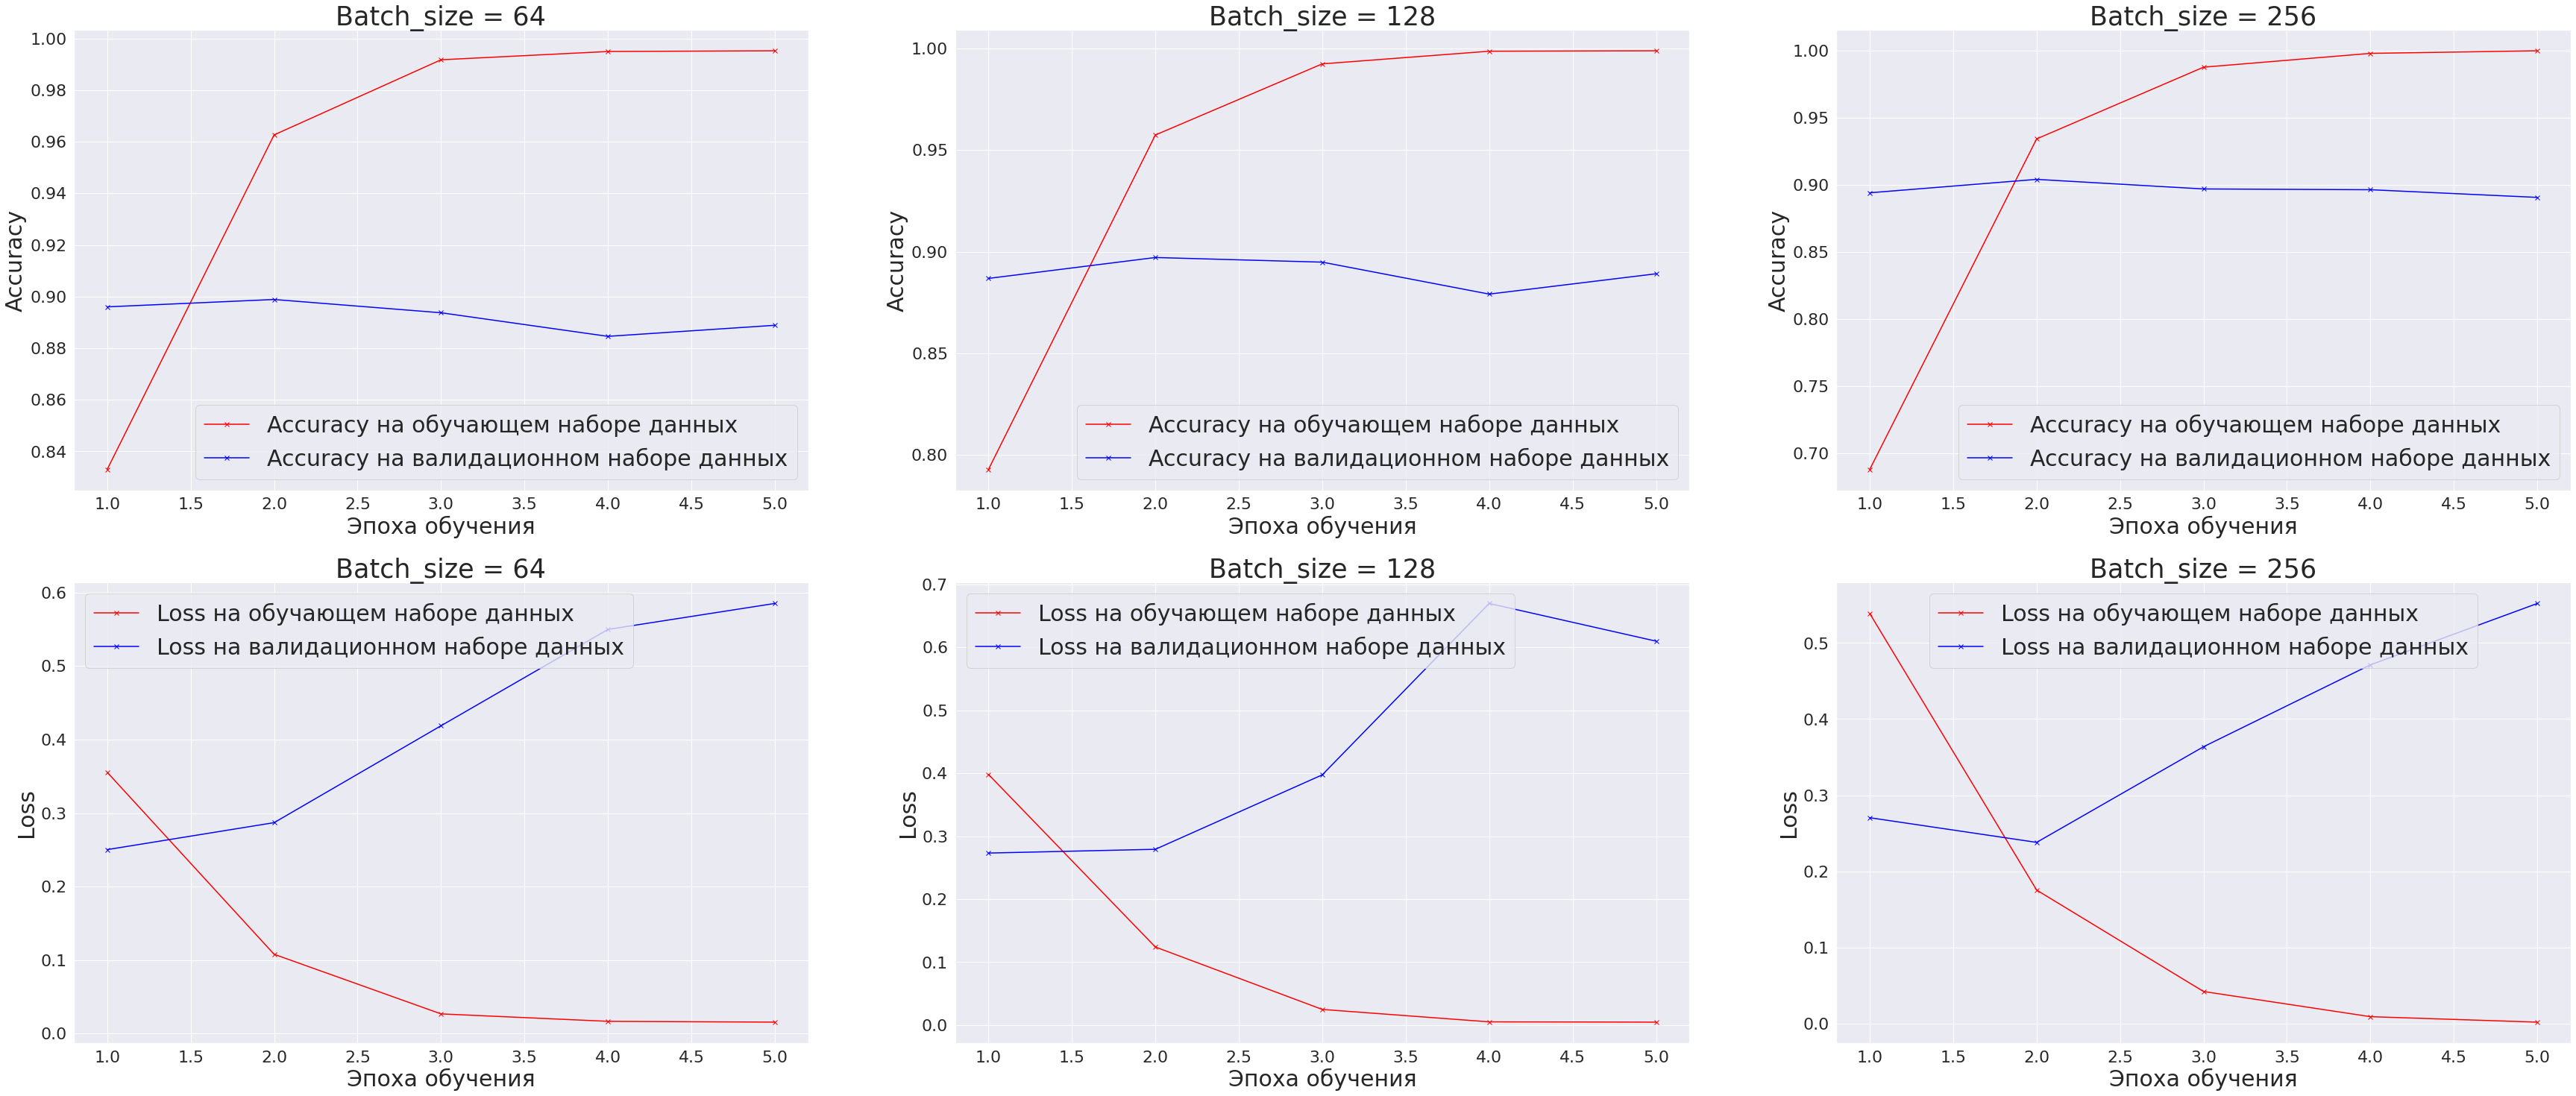
\includegraphics[scale=0.14]{cnn_batch.png}
    \caption{Поведение accuracy и loss в зависимости от batch size}
    \label{fig:cnn_batch}
\end{figure}
\begin{figure}[H]
    \centering
    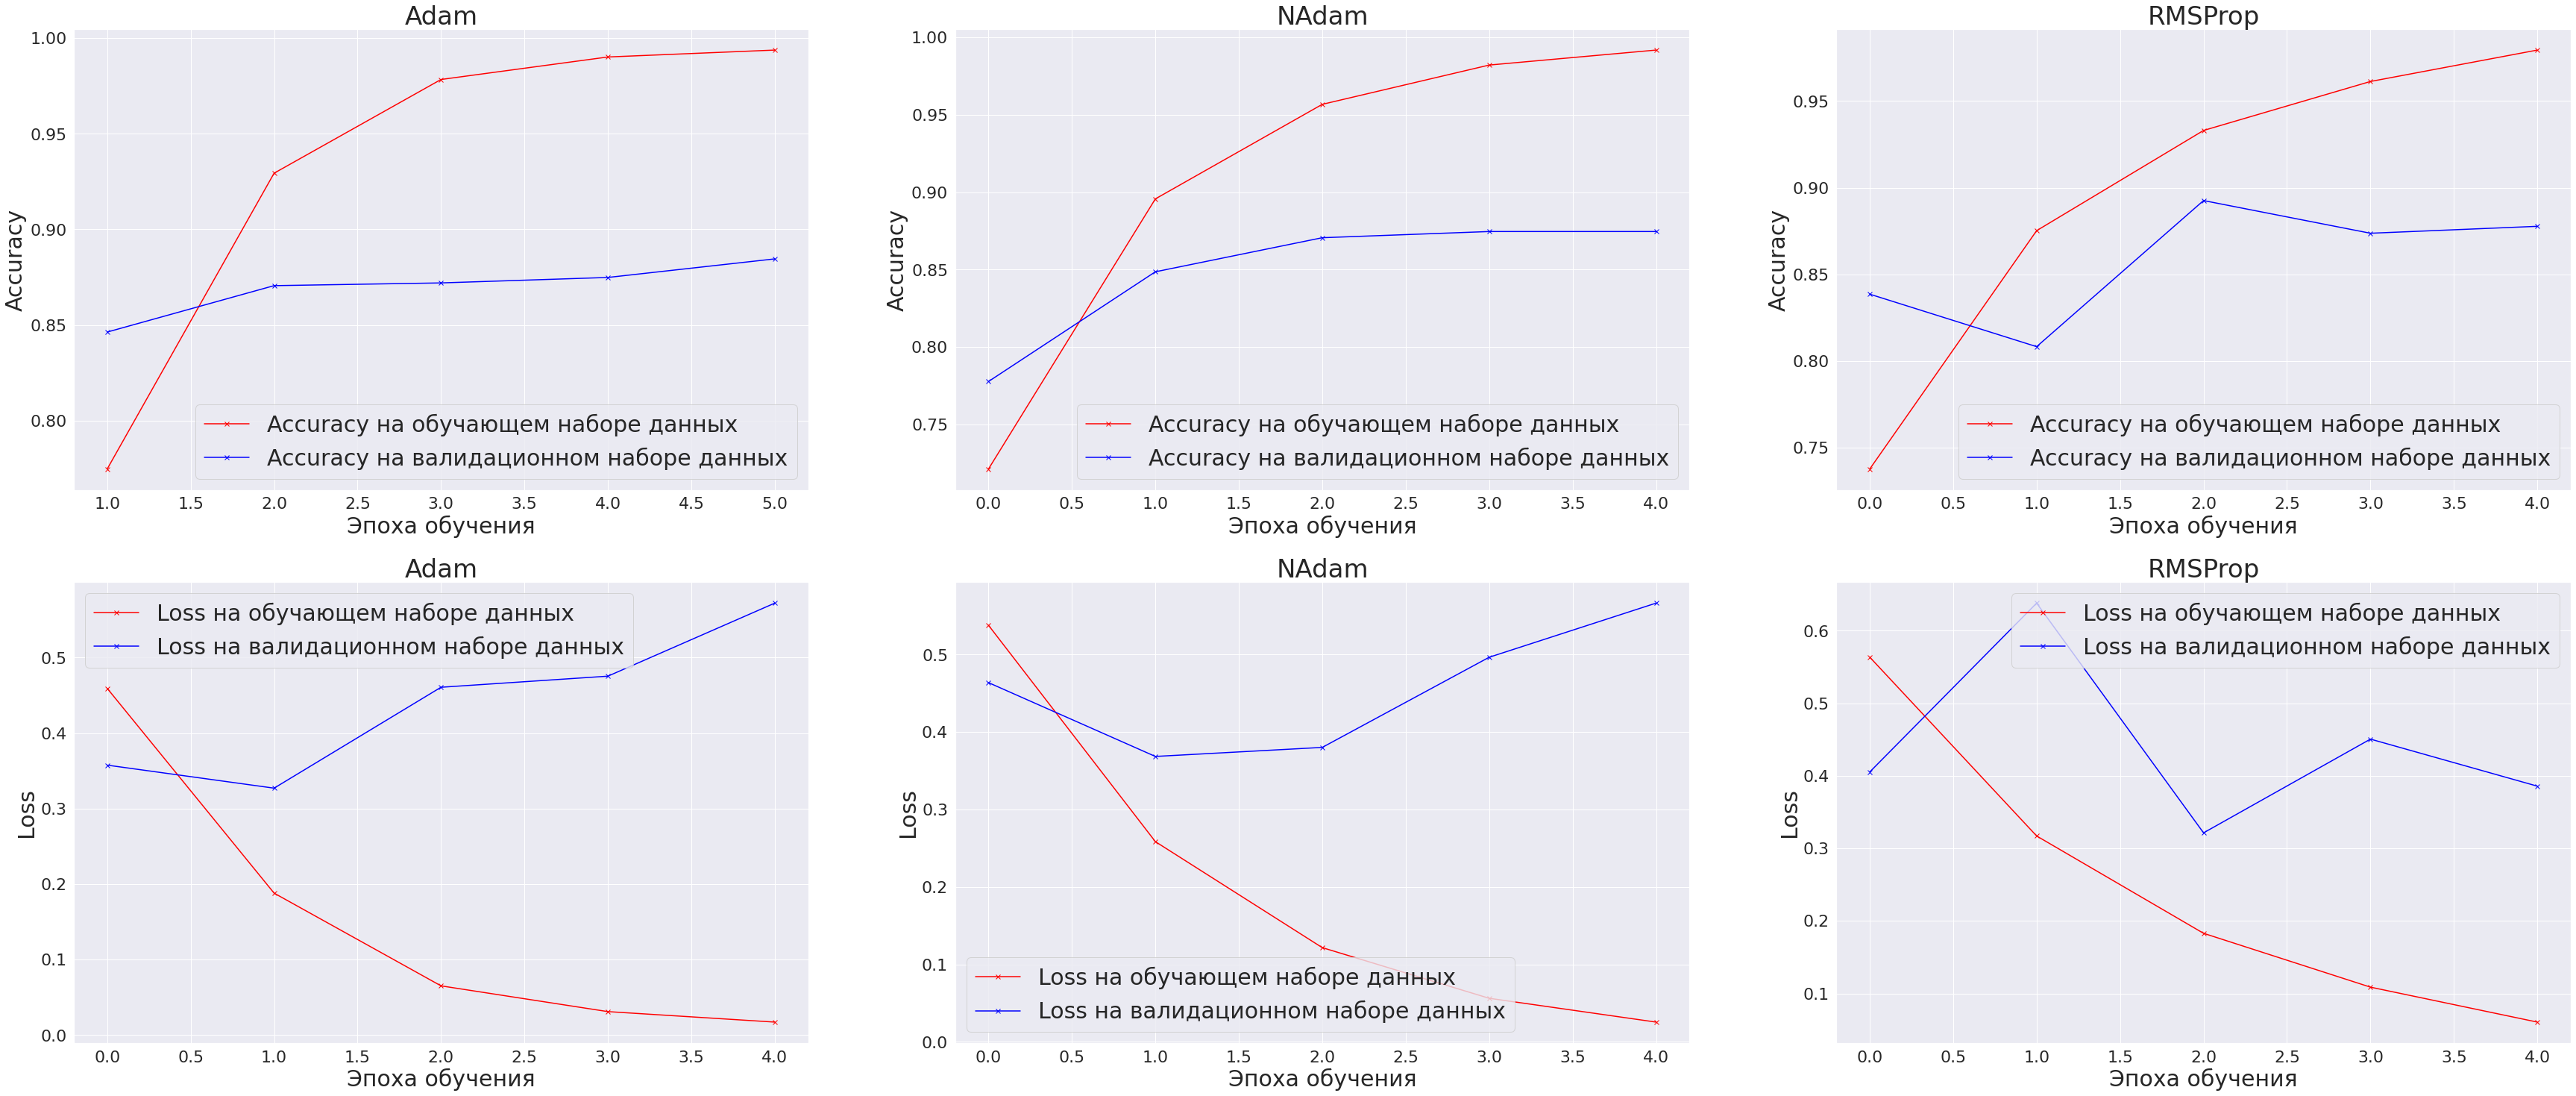
\includegraphics[scale=0.14]{cnn_optim.png}
    \caption{Поведение accuracy и loss в зависимости от выбора оптимизатора}
    \label{fig:cnn_optimizer}
\end{figure}
\subsubsection{Рекуррентные нейронные сети}
В Таблице \ref{tab:lstm_result1} приведены метрики качества accuracy исследуемых архитектур на этапах обучения, валидации и тестирования моделей. 
%accuracy lstm
\begin{center}
\begin{table}[H]
    \centering
    \caption{Метрика accuracy на разных этапах обучения}
    \resizebox{\textwidth}{!}{\begin{tabular}{|c|ccccccccc|}
    \hline
    \multirow{3}{*}{Данные}                               & \multicolumn{9}{c|}{Модели}                                                                                                                                                                                                                                                                                                           \\ \cline{2-10} 
                                                          & \multicolumn{3}{c|}{\begin{tabular}[c]{@{}c@{}}LSTM\\ (1 блок)\end{tabular}}                                      & \multicolumn{3}{c|}{\begin{tabular}[c]{@{}c@{}}LSTM\\ (2 блока)\end{tabular}}                            & \multicolumn{3}{c|}{\begin{tabular}[c]{@{}c@{}}CNN + LSTM\\ (1 слой + 1 пулинг + 1 блок)\end{tabular}} \\ \cline{2-10} 
                                                          & \multicolumn{1}{c|}{Train}           & \multicolumn{1}{c|}{Val}             & \multicolumn{1}{c|}{Test}           & \multicolumn{1}{c|}{Train}  & \multicolumn{1}{c|}{Val}             & \multicolumn{1}{c|}{Test}           & \multicolumn{1}{c|}{Train}              & \multicolumn{1}{c|}{Val}                & Test               \\ \hline
    \begin{tabular}[c]{@{}c@{}}IMDB\\ (2)\end{tabular}    & \multicolumn{1}{c|}{0.9968}          & \multicolumn{1}{c|}{0.8809}          & \multicolumn{1}{c|}{0.8573}         & \multicolumn{1}{c|}{0.9533} & \multicolumn{1}{c|}{\textbf{0.8834}} & \multicolumn{1}{c|}{0.8673}         & \multicolumn{1}{c|}{\textbf{0.9982}}    & \multicolumn{1}{c|}{0.88}               & \textbf{0.8765}    \\ \hline
    \begin{tabular}[c]{@{}c@{}}Twitter\\ (3)\end{tabular} & \multicolumn{1}{c|}{\textbf{0.855}}  & \multicolumn{1}{c|}{0.84}            & \multicolumn{1}{c|}{0.778}          & \multicolumn{1}{c|}{0.8431} & \multicolumn{1}{c|}{0.8393}          & \multicolumn{1}{c|}{\textbf{0.841}} & \multicolumn{1}{c|}{0.815}              & \multicolumn{1}{c|}{\textbf{0.8542}}    & 0.8175             \\ \hline
    \begin{tabular}[c]{@{}c@{}}Yelp\\ (2)\end{tabular}    & \multicolumn{1}{c|}{\textbf{0.9172}} & \multicolumn{1}{c|}{\textbf{0.9472}} & \multicolumn{1}{c|}{\textbf{0.945}} & \multicolumn{1}{c|}{0.91}   & \multicolumn{1}{c|}{0.864}           & \multicolumn{1}{c|}{0.8621}         & \multicolumn{1}{c|}{-}                  & \multicolumn{1}{c|}{\textbf{-}}         & -                  \\ \hline
    \multicolumn{1}{|l|}{Epochs}                          & \multicolumn{3}{c|}{13}                                                                                           & \multicolumn{3}{c|}{10}                                                                                  & \multicolumn{3}{c|}{10}                                                                                \\ \hline
    \end{tabular}}
    \label{tab:lstm_result1}
    \end{table}
\end{center}
%accuracy lstm
Таблица \ref{tab:lstm_result2} содержит сравнение современных фреймворков для обучения нейронных сетей PyTorch и Tensorflow. 
%time lstm
\begin{center}
\begin{table}[H]
    \centering
    \caption{Затраченное время на разных фреймворках}
    \resizebox{\textwidth}{!}{\begin{tabular}{|c|cccccc|c|}
    \hline
                                                          & \multicolumn{6}{c|}{Модели}                                                                                                                                                                        &                        \\ \hline
    \multirow{2}{*}{Данные}                               & \multicolumn{2}{c|}{\begin{tabular}[c]{@{}c@{}}LSTM\\ (1 блок)\end{tabular}} & \multicolumn{2}{c|}{\begin{tabular}[c]{@{}c@{}}LSTM\\ (2 блока)\end{tabular}} & \multicolumn{2}{c|}{LSTM + CNN}     & \multirow{2}{*}{Объем} \\ \cline{2-7}
                                                          & \multicolumn{1}{c|}{TF}              & \multicolumn{1}{c|}{PyTorch}          & \multicolumn{1}{c|}{TF}               & \multicolumn{1}{c|}{PyTorch}          & \multicolumn{1}{c|}{TF}   & PyTorch &                        \\ \hline
    \begin{tabular}[c]{@{}c@{}}IMDB\\ (2)\end{tabular}    & \multicolumn{1}{c|}{225}             & \multicolumn{1}{c|}{201}              & \multicolumn{1}{c|}{8400}             & \multicolumn{1}{c|}{8513}             & \multicolumn{1}{c|}{1800} & 1680    & 50000                  \\ \hline
    \begin{tabular}[c]{@{}c@{}}Twitter\\ (3)\end{tabular} & \multicolumn{1}{c|}{541}             & \multicolumn{1}{c|}{650}              & \multicolumn{1}{c|}{28326}            & \multicolumn{1}{c|}{31652}            & \multicolumn{1}{c|}{3366} & 3254    & 75000                  \\ \hline
    \begin{tabular}[c]{@{}c@{}}Yelp\\ (2)\end{tabular}    & \multicolumn{1}{c|}{432002}          & \multicolumn{1}{c|}{542331}           & \multicolumn{1}{c|}{479032}           & \multicolumn{1}{c|}{482151}           & \multicolumn{1}{c|}{-}    & -       & 560000                 \\ \hline
    \end{tabular}}
    \label{tab:lstm_result2}
    \end{table}
\end{center}
%time lstm
На рис. \ref{fig:lstm_batch} и рис. \ref{fig:cnn_optimizer} изображены поведения ошибки и метрики качества в зависимости от выбора размера пакета и оптимизатора, соответственно.
\begin{figure}[H]
    \centering
    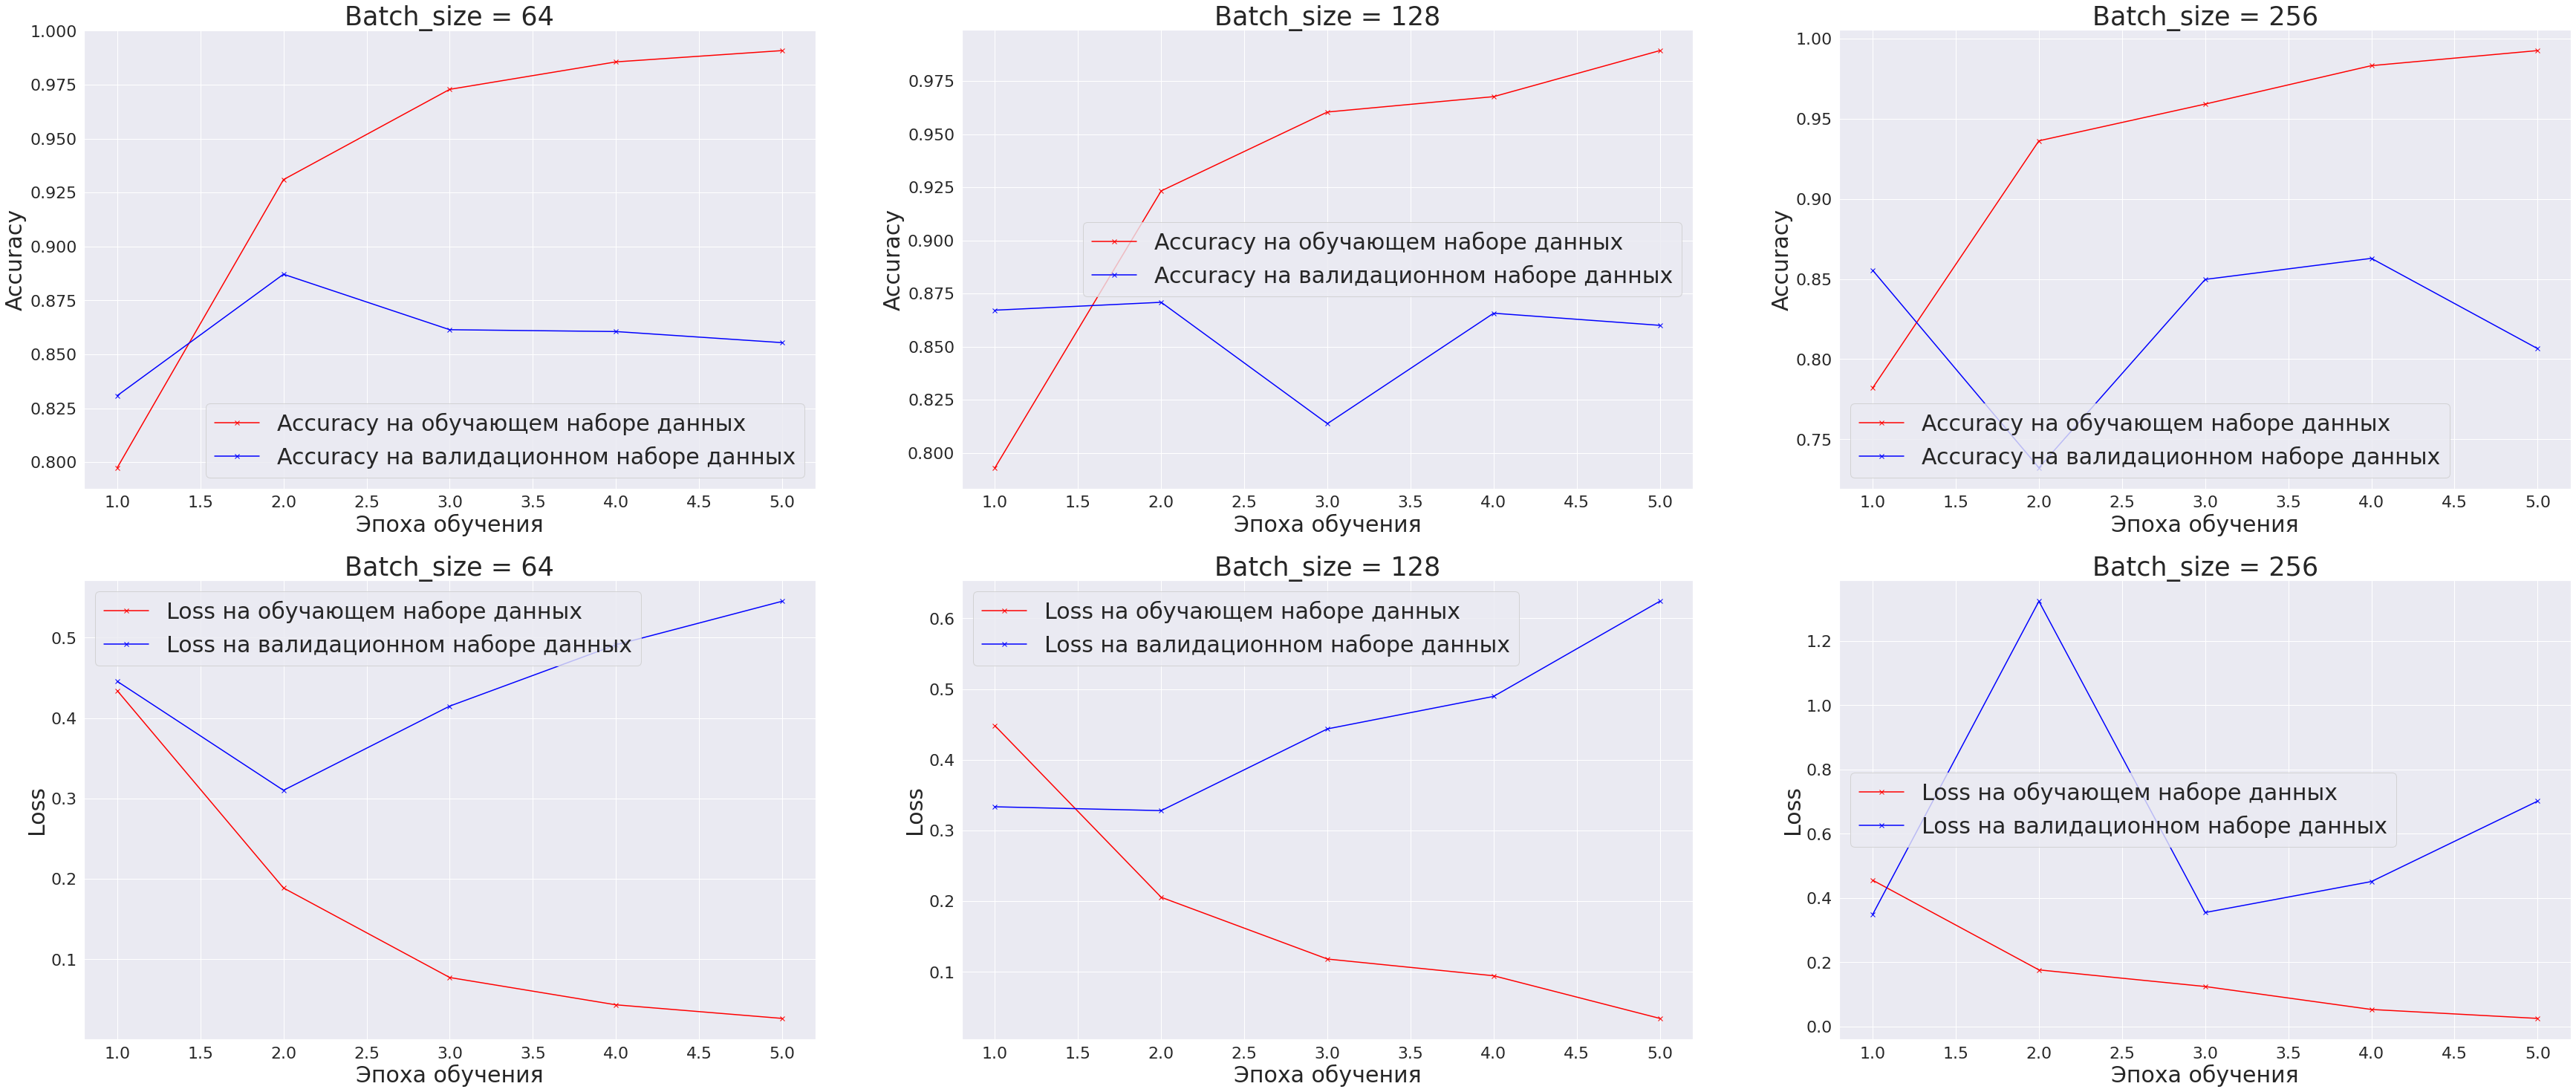
\includegraphics[scale=0.14]{lstm_batch.png}
    \caption{Поведение accuracy и loss в зависимости от batch size}
    \label{fig:lstm_batch}
\end{figure}
\begin{figure}[H]
    \centering
    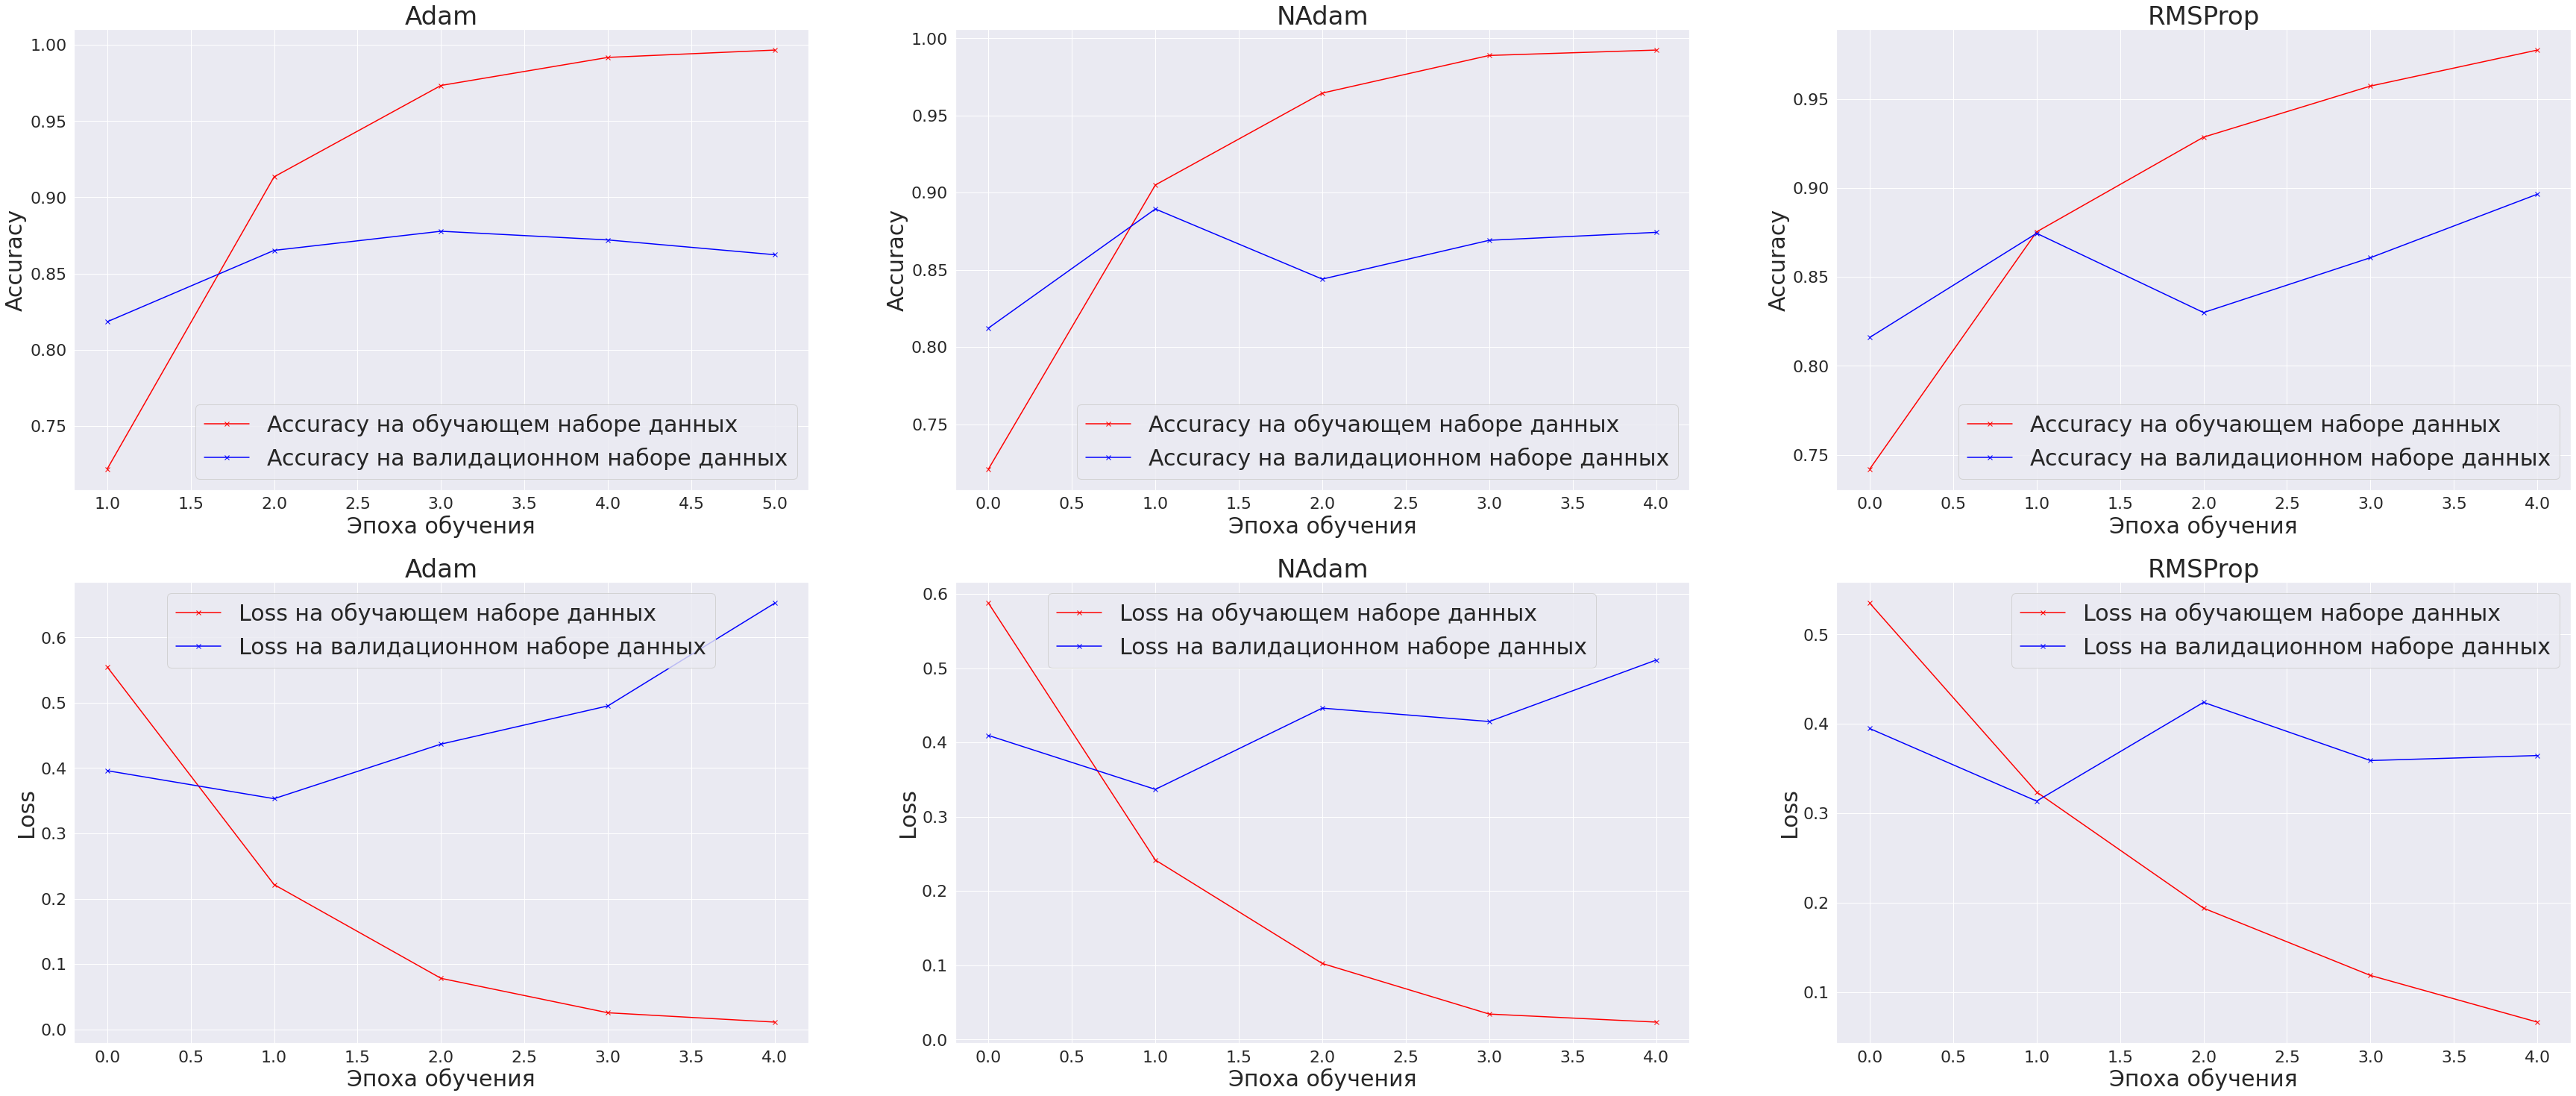
\includegraphics[scale=0.14]{lstm_optim.png}
    \caption{Поведение accuracy и loss в зависимости от выбора оптимизатора}
    \label{fig:lstm_optimizer}
\end{figure}
В Таблице \ref{tab:gru_result1} приведены метрики качества accuracy исследуемых архитектур на этапах обучения, валидации и тестирования моделей. 
%accuracy gru
\begin{center}
    % Please add the following required packages to your document preamble:
% \usepackage{multirow}
\begin{table}[H]
    \centering
    \caption{Метрика accuracy на разных этапах обучения}
    \resizebox{\textwidth}{!}{\begin{tabular}{|c|ccccccccc|}
    \hline
    \multirow{3}{*}{Данные}                               & \multicolumn{9}{c|}{Модели}                                                                                                                                                                                                                                                                                          \\ \cline{2-10} 
                                                          & \multicolumn{3}{c|}{\begin{tabular}[c]{@{}c@{}}GRU\\ (1 блок)\end{tabular}}                                        & \multicolumn{3}{c|}{\begin{tabular}[c]{@{}c@{}}GRU\\ (2 блока)\end{tabular}}            & \multicolumn{3}{c|}{\begin{tabular}[c]{@{}c@{}}CNN + GRU\\ (5 слой + 5 пулинг + 1 блок)\end{tabular}} \\ \cline{2-10} 
                                                          & \multicolumn{1}{c|}{Train}           & \multicolumn{1}{c|}{Val}             & \multicolumn{1}{c|}{Test}            & \multicolumn{1}{c|}{Train}  & \multicolumn{1}{c|}{Val}    & \multicolumn{1}{c|}{Test}   & \multicolumn{1}{c|}{Train}              & \multicolumn{1}{c|}{Val}               & Test               \\ \hline
    \begin{tabular}[c]{@{}c@{}}IMDB\\ (2)\end{tabular}    & \multicolumn{1}{c|}{0.9751}          & \multicolumn{1}{c|}{\textbf{0.9612}} & \multicolumn{1}{c|}{\textbf{0.9353}} & \multicolumn{1}{c|}{0.9903} & \multicolumn{1}{c|}{0.8764} & \multicolumn{1}{c|}{0.8931} & \multicolumn{1}{c|}{\textbf{0.9969}}    & \multicolumn{1}{c|}{0.8851}            & 0.9185             \\ \hline
    \begin{tabular}[c]{@{}c@{}}Twitter\\ (3)\end{tabular} & \multicolumn{1}{c|}{0.8788}          & \multicolumn{1}{c|}{0.8338}          & \multicolumn{1}{c|}{0.8447}          & \multicolumn{1}{c|}{0.9937} & \multicolumn{1}{c|}{0.9605} & \multicolumn{1}{c|}{0.9574} & \multicolumn{1}{c|}{0.93}               & \multicolumn{1}{c|}{\textbf{0.872}}    & \textbf{0.8771}    \\ \hline
    \begin{tabular}[c]{@{}c@{}}Yelp\\ (2)\end{tabular}    & \multicolumn{1}{c|}{\textbf{0.9670}} & \multicolumn{1}{c|}{\textbf{0.9562}} & \multicolumn{1}{c|}{\textbf{0.9459}} & \multicolumn{1}{c|}{0.954}  & \multicolumn{1}{c|}{0.943}  & \multicolumn{1}{c|}{0.9126} & \multicolumn{1}{c|}{-}                  & \multicolumn{1}{c|}{\textbf{-}}        & -                  \\ \hline
    \multicolumn{1}{|l|}{Epochs}                          & \multicolumn{3}{c|}{5}                                                                                             & \multicolumn{3}{c|}{5}                                                                  & \multicolumn{3}{c|}{5}                                                                                \\ \hline
    \end{tabular}}
    \label{tab:gru_result1}
    \end{table}
\end{center}
%accuracy gru
Таблица \ref{tab:gru_result2} содержит сравнение современных фреймворков для обучения нейронных сетей PyTorch и Tensorflow. 
В ней приведены длительности обучения моделей. 
%time gru
\begin{center}
    \begin{table}[H]
        \caption{Затраченное время на разных фреймворках}
        \resizebox{\textwidth}{!}{\begin{tabular}{|c|cccccc|c|}
        \hline
                                                              & \multicolumn{6}{c|}{Модели}                                                                                                                                                                      &                        \\ \hline
        \multirow{2}{*}{Данные}                               & \multicolumn{2}{c|}{\begin{tabular}[c]{@{}c@{}}GRU\\ (1 блок)\end{tabular}} & \multicolumn{2}{c|}{\begin{tabular}[c]{@{}c@{}}GRU \\ (2 блока)\end{tabular}} & \multicolumn{2}{c|}{GRU + CNN}     & \multirow{2}{*}{Объем} \\ \cline{2-7}
                                                              & \multicolumn{1}{c|}{TF}              & \multicolumn{1}{c|}{PyTorch}         & \multicolumn{1}{c|}{TF}               & \multicolumn{1}{c|}{PyTorch}          & \multicolumn{1}{c|}{TF}  & PyTorch &                        \\ \hline
        \begin{tabular}[c]{@{}c@{}}IMDB\\ (2)\end{tabular}    & \multicolumn{1}{c|}{189}             & \multicolumn{1}{c|}{204}             & \multicolumn{1}{c|}{569}              & \multicolumn{1}{c|}{642}              & \multicolumn{1}{c|}{244} & 183     & 50000                  \\ \hline
        \begin{tabular}[c]{@{}c@{}}Twitter\\ (3)\end{tabular} & \multicolumn{1}{c|}{546}             & \multicolumn{1}{c|}{498}             & \multicolumn{1}{c|}{759}              & \multicolumn{1}{c|}{802}              & \multicolumn{1}{c|}{650} & 663     & 75000                  \\ \hline
        \begin{tabular}[c]{@{}c@{}}Yelp\\ (2)\end{tabular}    & \multicolumn{1}{c|}{433200}          & \multicolumn{1}{c|}{454233}          & \multicolumn{1}{c|}{679036}           & \multicolumn{1}{c|}{592431}           & \multicolumn{1}{c|}{-}   & -       & 560000                 \\ \hline
        \end{tabular}}
        \label{tab:gru_result2}
        \end{table}
\end{center}
%time gru
На рис. \ref{fig:gru_batch} и рис. \ref{fig:gru_optimizer} изображены поведения ошибки и метрики качества в зависимости от выбора размера пакета и оптимизатора, соответственно.
\begin{figure}[H]
    \centering
    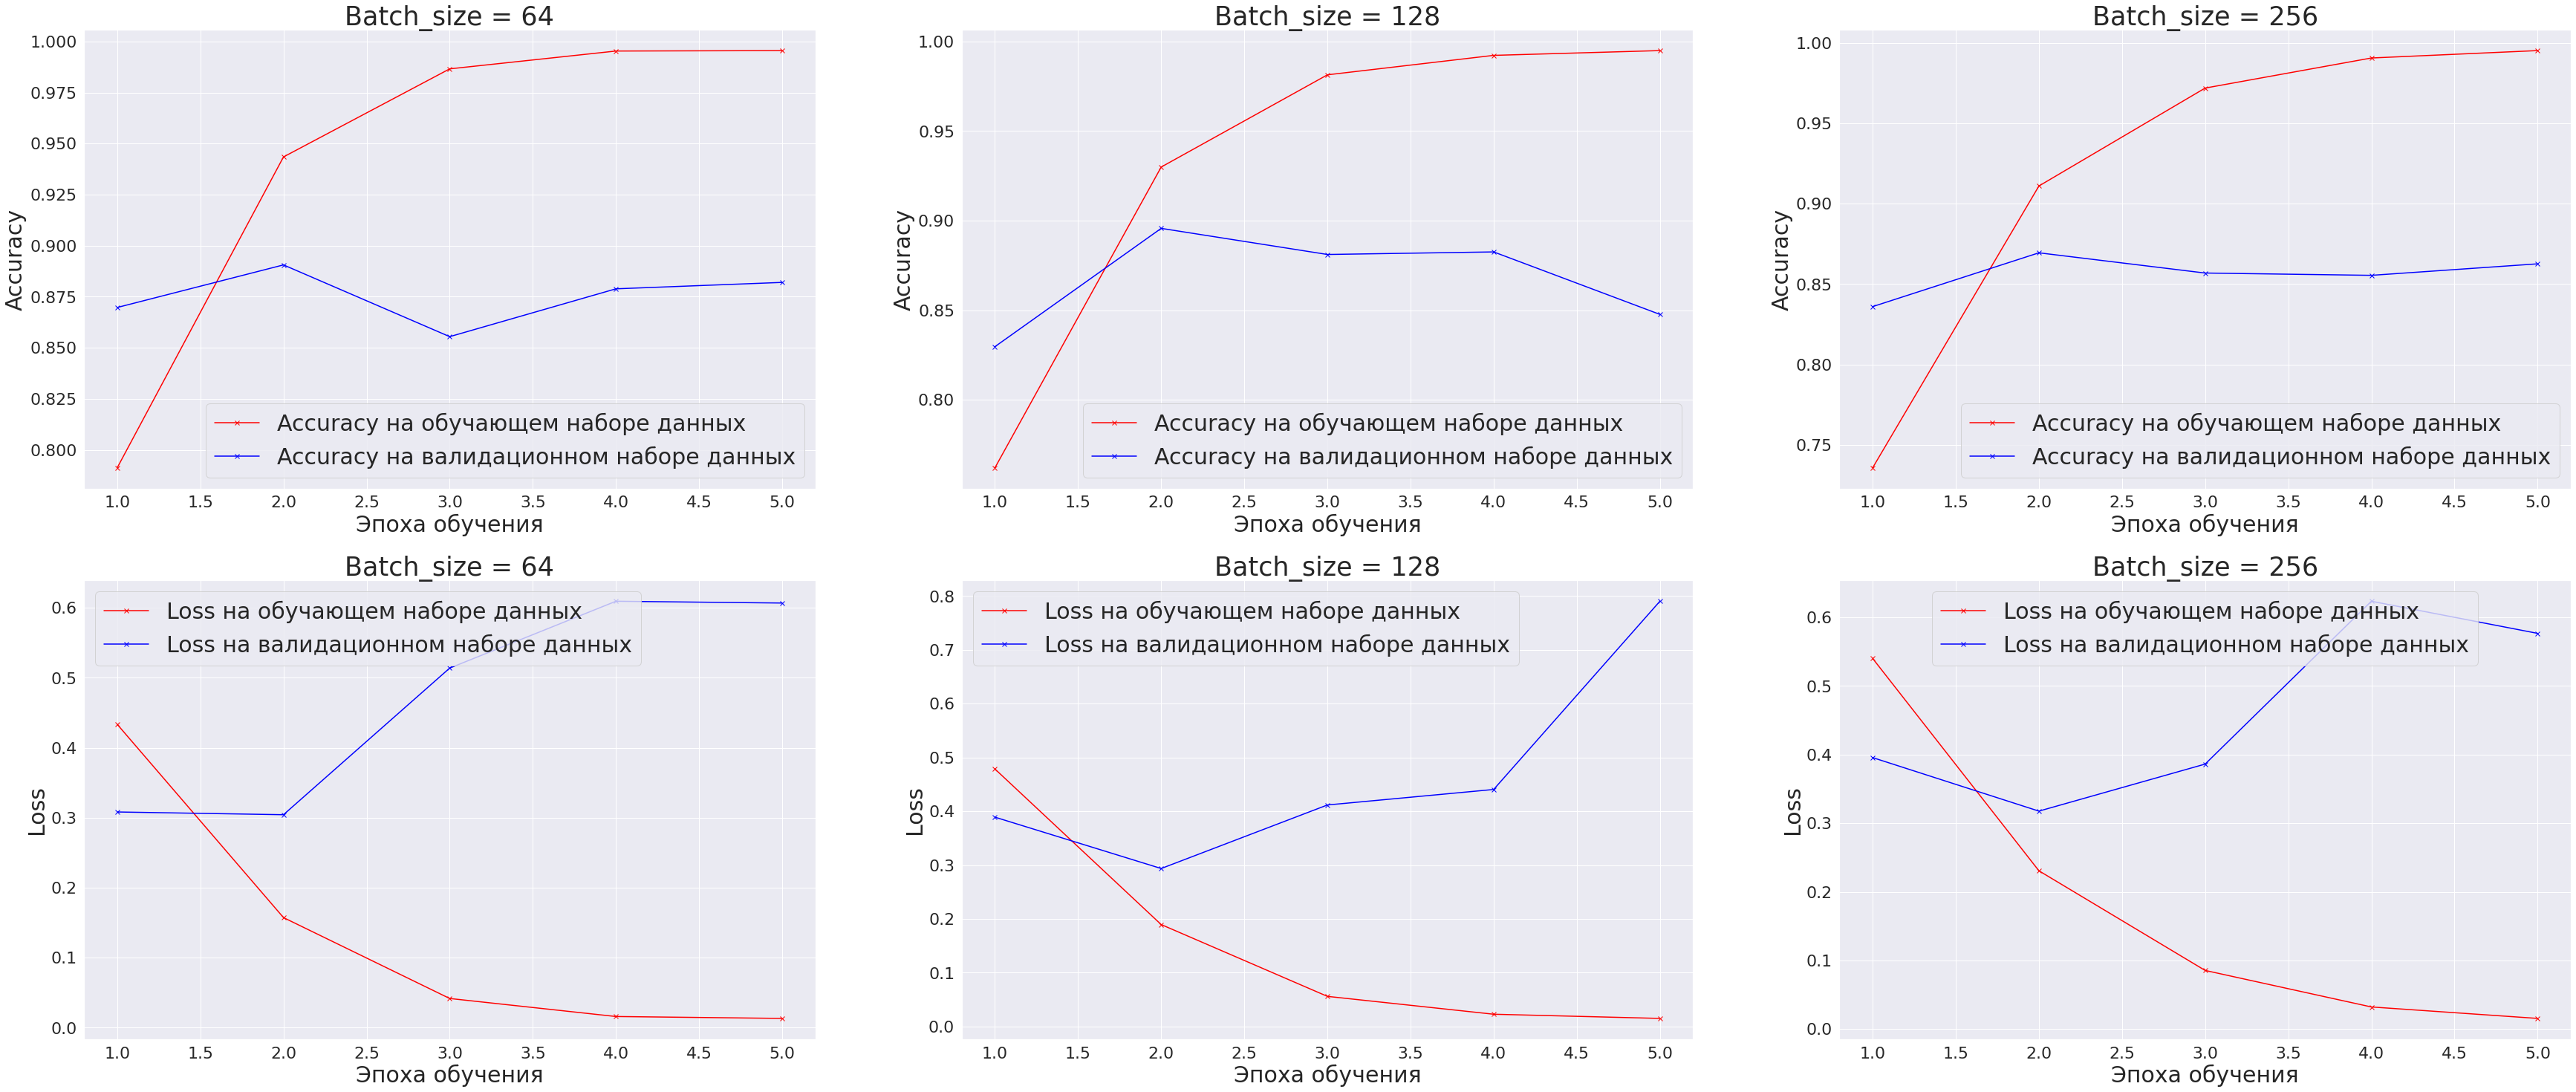
\includegraphics[scale=0.14]{gru_batch.png}
    \caption{Поведение accuracy и loss в зависимости от batch size}
    \label{fig:gru_batch}
\end{figure}
\begin{figure}[H]
    \centering
    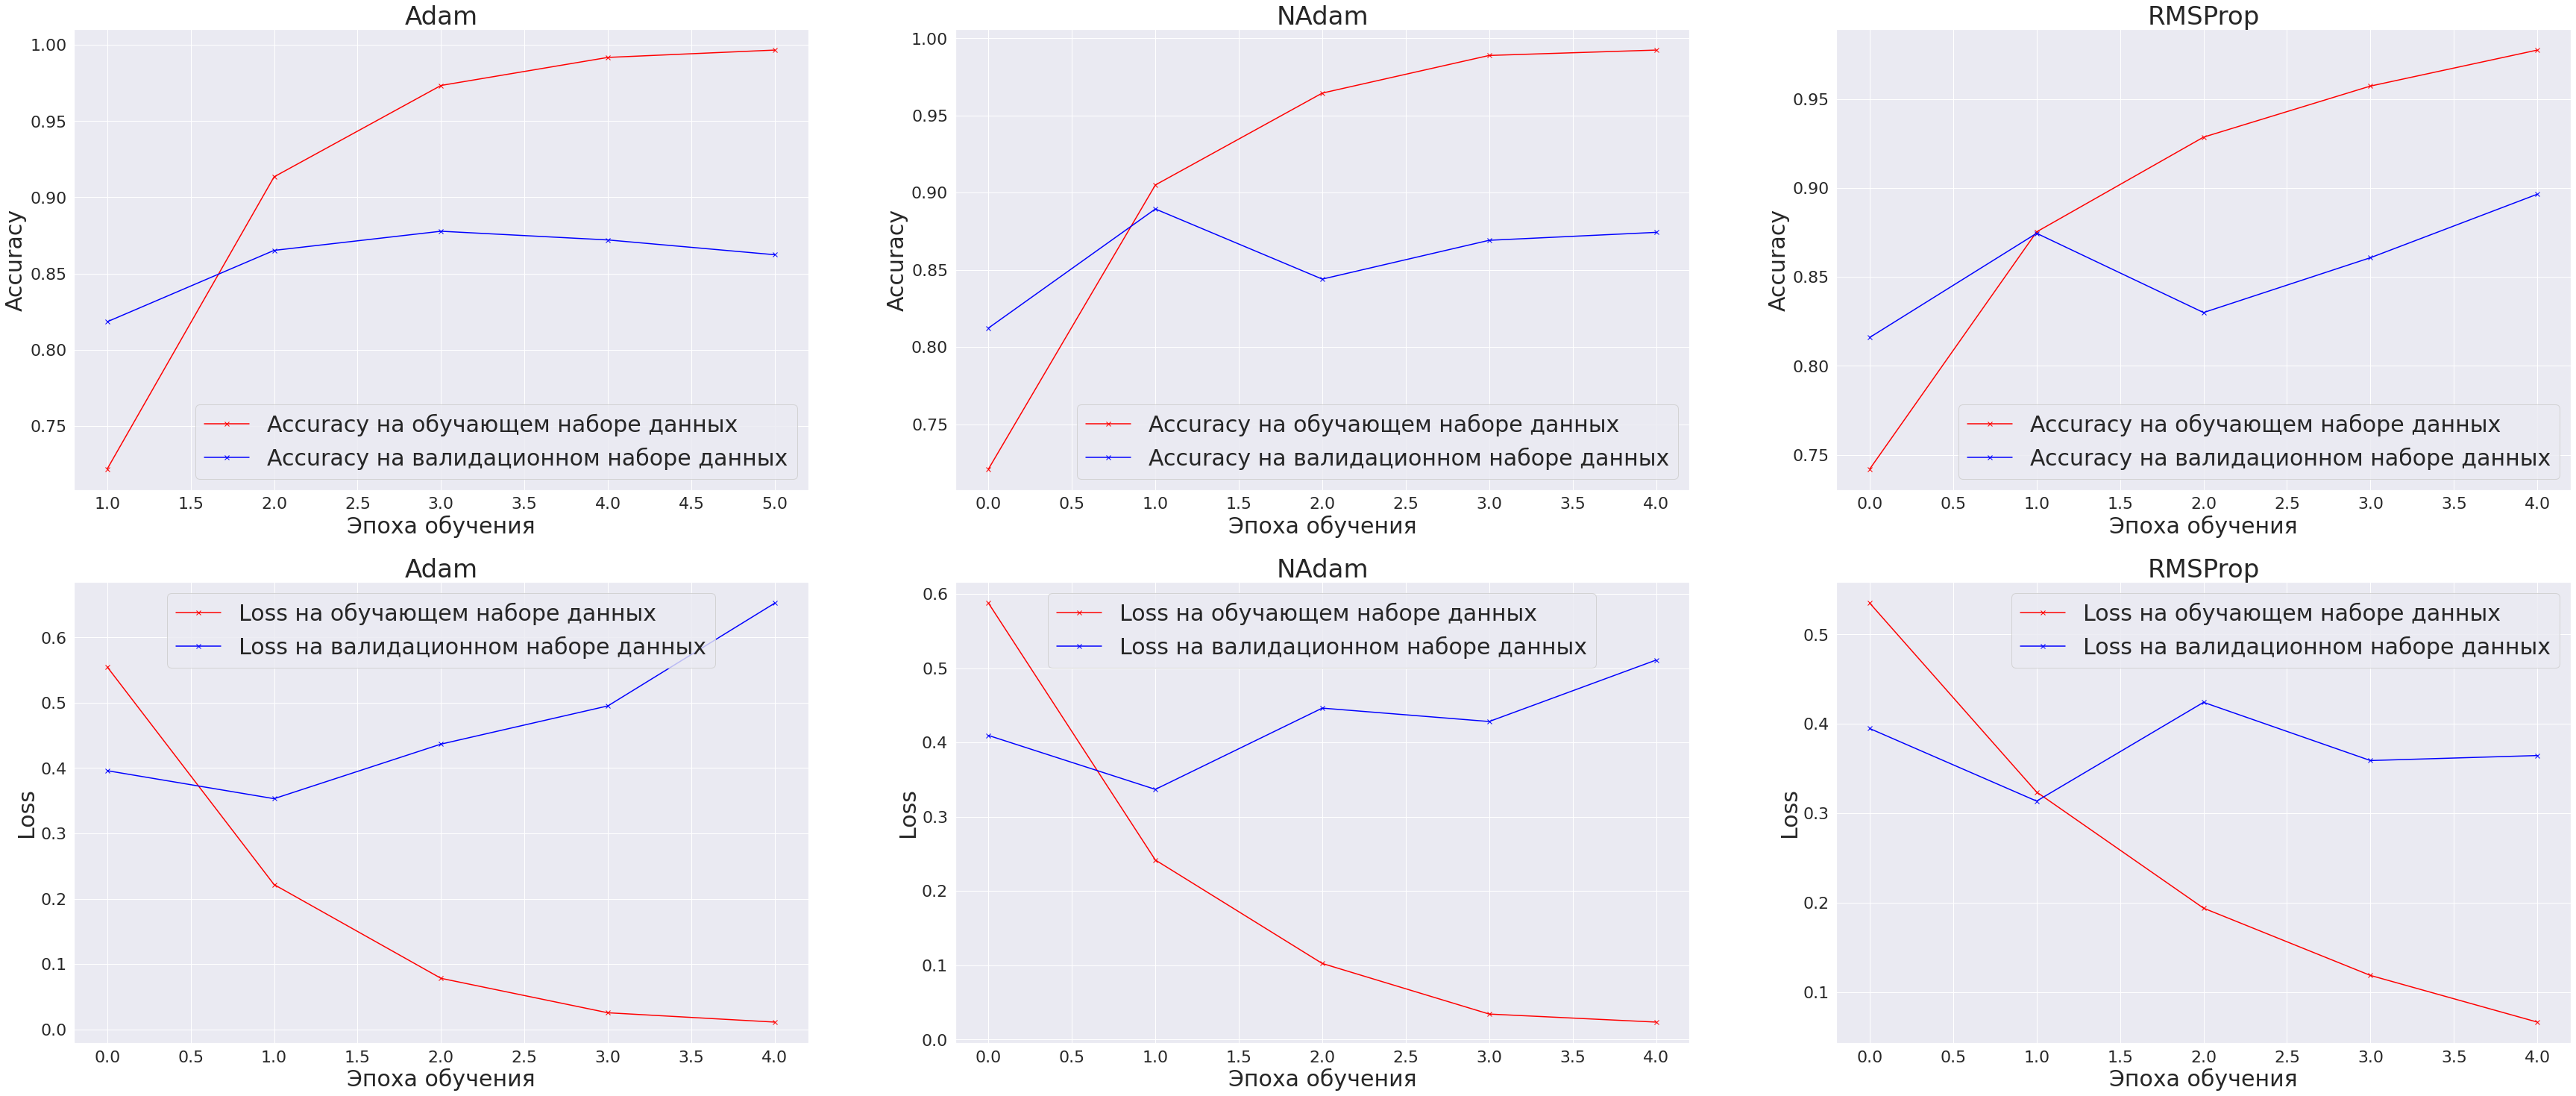
\includegraphics[scale=0.14]{gru_optim.png}
    \caption{Поведение accuracy и loss в зависимости от выбора оптимизатора}
    \label{fig:gru_optimizer}
\end{figure}
Embedding-слой, как и предполагалось, показал лучший результат по сравнению с предобученными моделями Word2Vec (Таблица \ref{tab:embeddings}), однако, разница невелика, поэтому можно сделать вывод, что в промышленной разработке следует использовать последний в силу большего по объемам латентного словаря (если нет ограничений по памяти).
    \begin{table}[H]
    \begin{center}
\caption{Сравнение различных векторных представлений слов}
\scalebox{0.87}[0.87]{\begin{tabular}{|l|ccc|}
\hline
                                                               & \multicolumn{3}{c|}{Модели}                                                                                                               \\ \cline{2-4} 
\multirow{-2}{*}{Эмбеддинги}                                   & \multicolumn{1}{c|}{CNN}                            & \multicolumn{1}{c|}{LSTM}                          & GRU                            \\ \hline
W2V CBOW                                                       & \multicolumn{1}{c|}{0.8991}                         & \multicolumn{1}{c|}{0.88}                          & 0.9353                         \\ \hline
W2V Skip-gram                                                  & \multicolumn{1}{c|}{\textbf{0.8771}} & \multicolumn{1}{c|}{\textbf{0.841}} & \textbf{0.9574} \\ \hline
\begin{tabular}[c]{@{}l@{}}Trainable \\ embedding\end{tabular} & \multicolumn{1}{c|}{0.9012}                         & \multicolumn{1}{c|}{0.9172}                        & 0.9562                         \\ \hline
\end{tabular}}
\label{tab:embeddings}
\end{center}
\end{table}
\subsubsection{Приемы мета-моделирования}
Полученные обученные модели показывают хорошие результаты, однако их можно дополнительно улучшить с помощью технологий стэкинга. Идея заключается в создании метамодели, которая будет по результатам мета-признаков моделей давать конечное предсказание. Обучение моделей для создания мета-модели проходило по принципу Stratified K-Foldation с сохранением балансировки классов (рис. \ref{fig:kfold}).  
\begin{figure}[H]
    \centering
    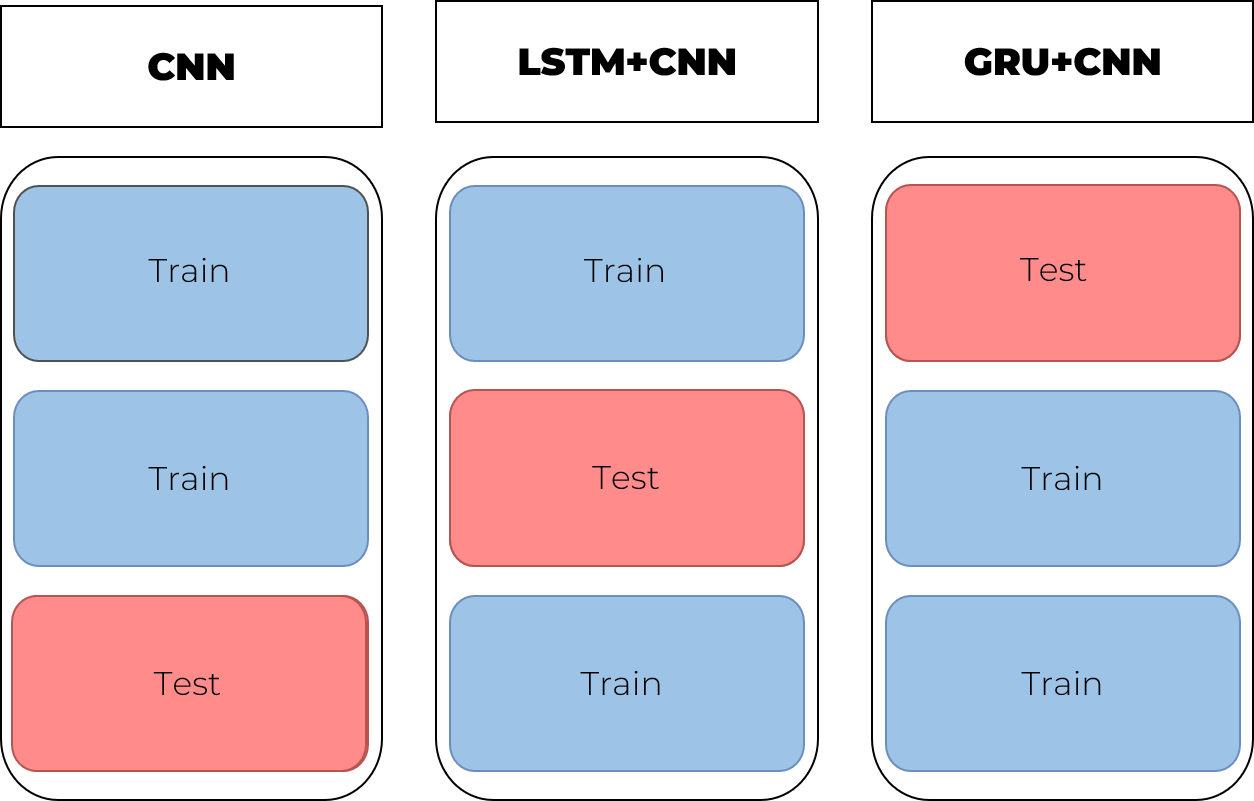
\includegraphics[scale=0.5]{Kfold.png}
    \caption{Stratified K-Foldation для мета моделирования}
    \label{fig:kfold}
\end{figure}
Тренировочный датасет объемом 3.625 миллионов отзывов (результат присоединения датасетов Amazon и IMDB), был разбит на три части, на двух из которых каждая модель обучалась, затем у нее убирался полносвязный слой с sigmoid функцией активации, чтобы получить признаковое описание начальных данных сложной структуры в виде табличной структуры, а на третьей части каждая модель давала предсказания без пересечения между собой. Мета-предсказания, будучи табличными данными, были 
адресованы в классификаторы Random Forest, GBM, SVM, обученные по принципу кросс-валидации (рис. \ref{fig:crossval})
\begin{figure}[H]
    \centering
    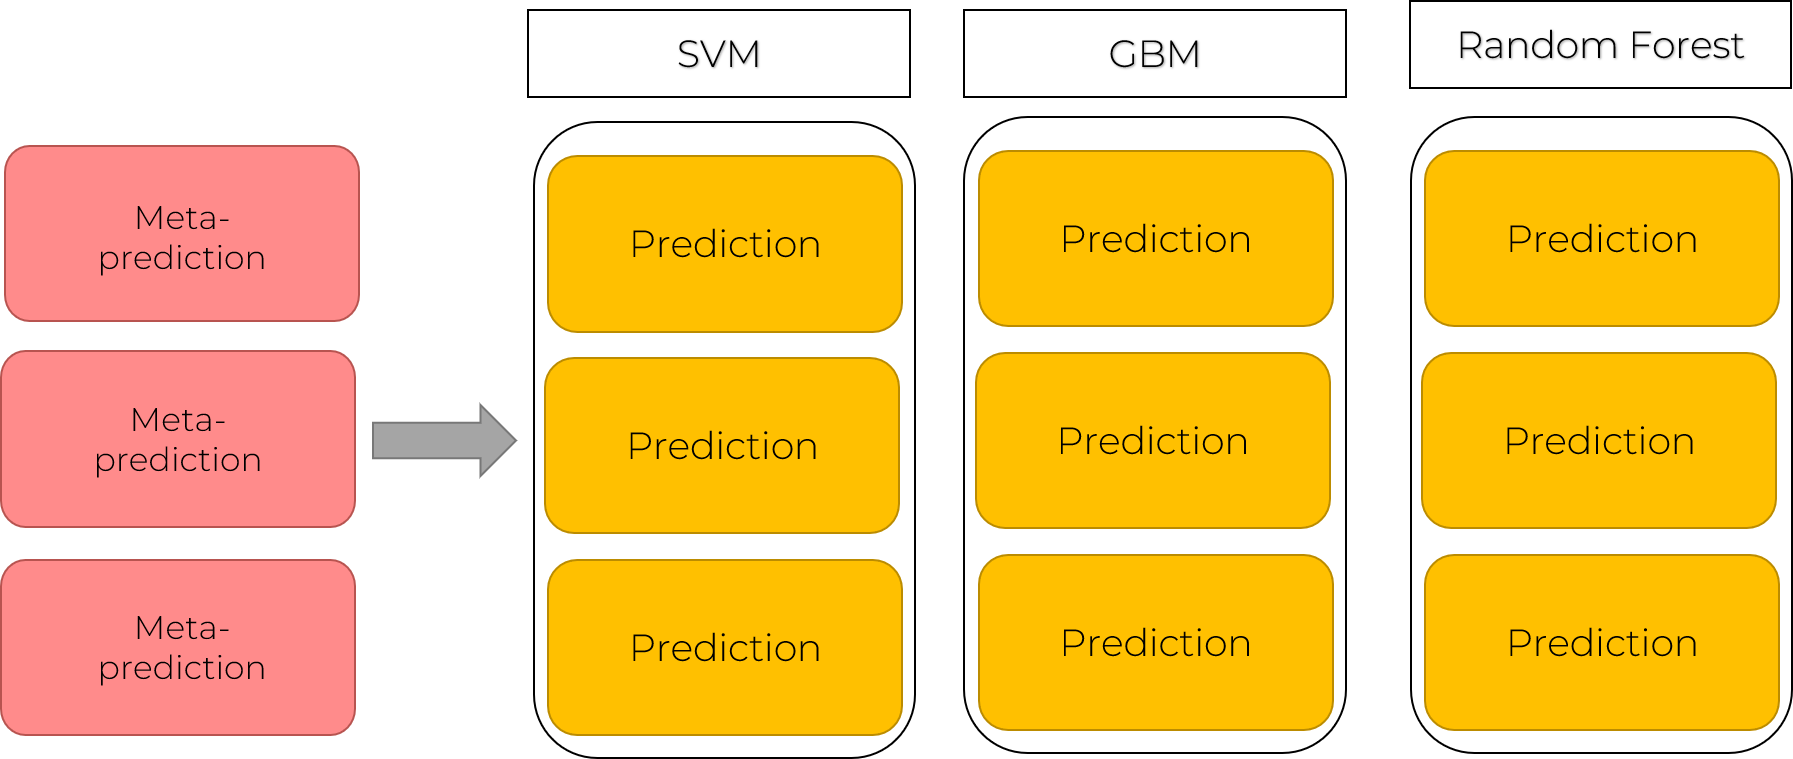
\includegraphics[scale=0.5]{meta.png}
    \caption{Кроссвалидация ансамблированных моделей}
    \label{fig:crossval}
\end{figure}
Усредненный результат трех предсказательных моделей является конечным результатом (рис. \ref{fig:postmeta}):
\begin{figure}[H]
    \centering
    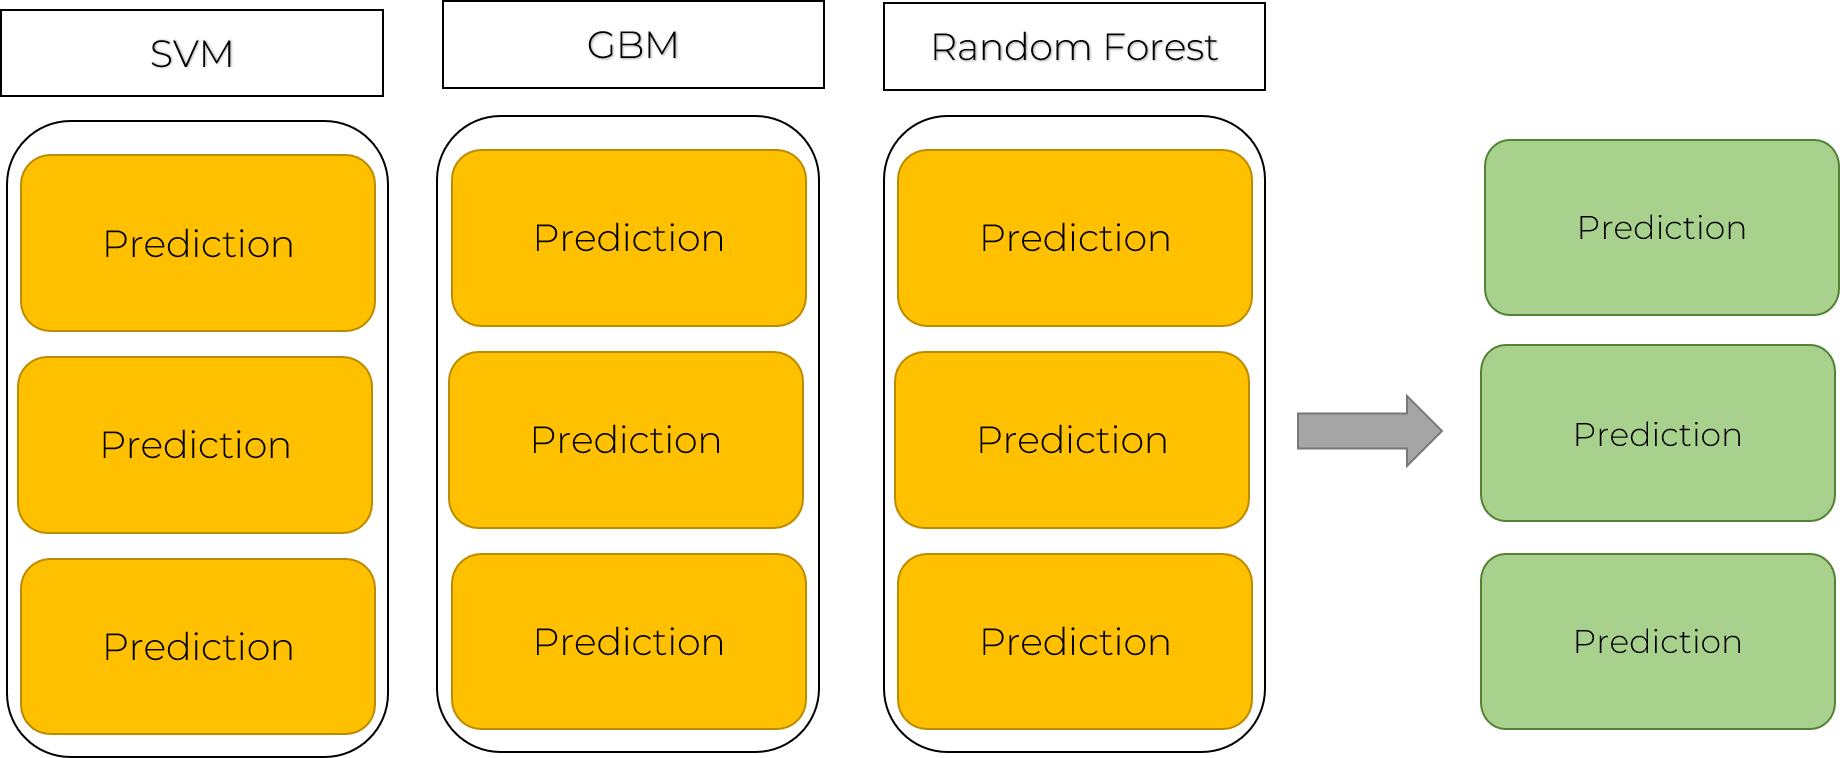
\includegraphics[scale=0.5]{postmeta.png}
    \caption{Ансамблирование и голосование}
    \label{fig:postmeta}
\end{figure}
\subsubsection{Реализация веб-сервиса}
\paragraph{Скраппинг}
\par
Для реализации веб-сервиса по анализу общественного мнения в видеохостинге YouTube были написаны скрапперы с помощью Selenium и Youtube API (так как время работы прототипа с использованием системы автоматизации Selenium было излишне долгим). В рамках Selenium собирается информация о видео (так как это не требует скроллинга) и асинхронно с этим происходит запрос в YouTube API с целью собрать комментарии, количество лайков и ответов на эти комментарии. Затем наскраппленные данные направляются в обученные модели, логиты с последнего слоя которых подаются в классификаторы машинного обучение, затем результат усредняется. Такой же подход был реализован в статье, представляемой в \cite{gagar} с реализацией телеграм-бота. 
\paragraph{Frontend разработка}
В качестве шаблона был использован Bootstrap5 и Jinja2 в качестве шаблонизатора. Верстка шаблонов страниц проделана с помощью HTML и CSS. В рамках работы были произведены масштабирование и адаптация под разные экраны пользователей. Можно говорить о кросс-платформенном использовании web-приложения.
\paragraph{Backend разработка}
В качестве серверной части web-приложения использован фреймворк Flask и локальное хранение данных.
\paragraph{Визуализация}
Главная страница сервиса с навигацией рис. \ref{fig:web1}, \ref{fig:web2}:
\begin{figure}[H]
    \centering
    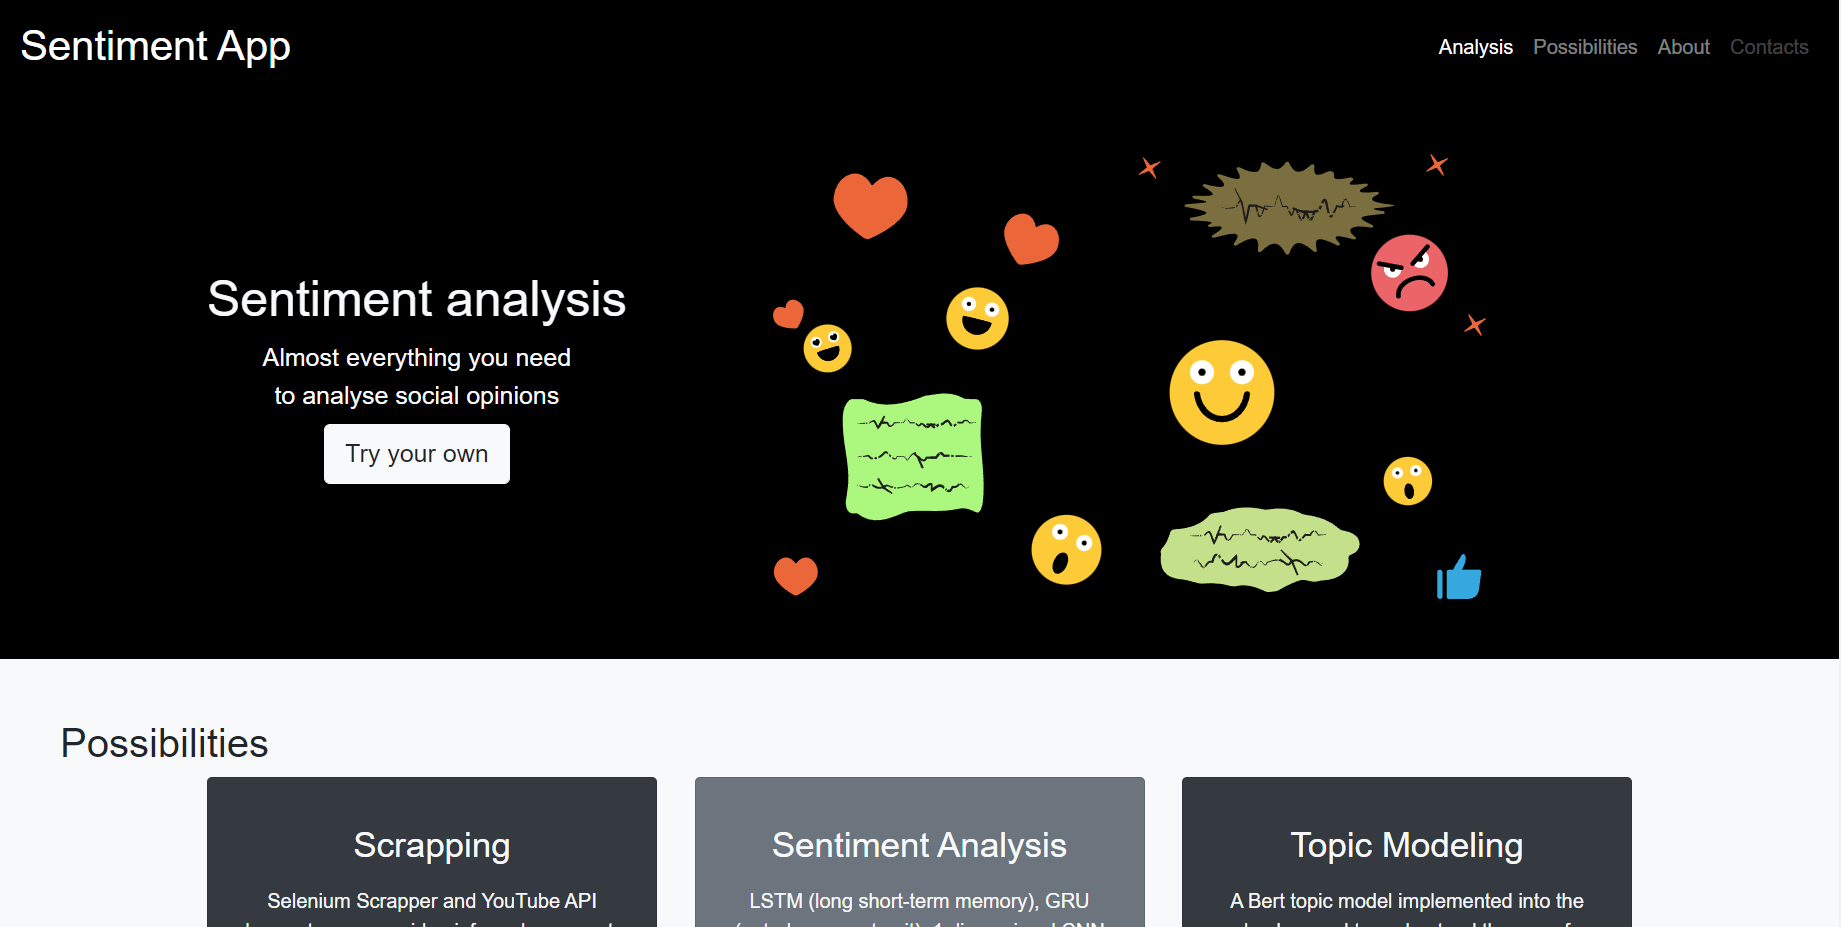
\includegraphics[scale=0.4]{web1.png}
    \caption{Главная страница сервиса}
    \label{fig:web1}
\end{figure}
В поле Link можно вставить ссылку на видео YouTube и запустить таким образом процесс анализа: 
\begin{figure}[H]
    \centering
    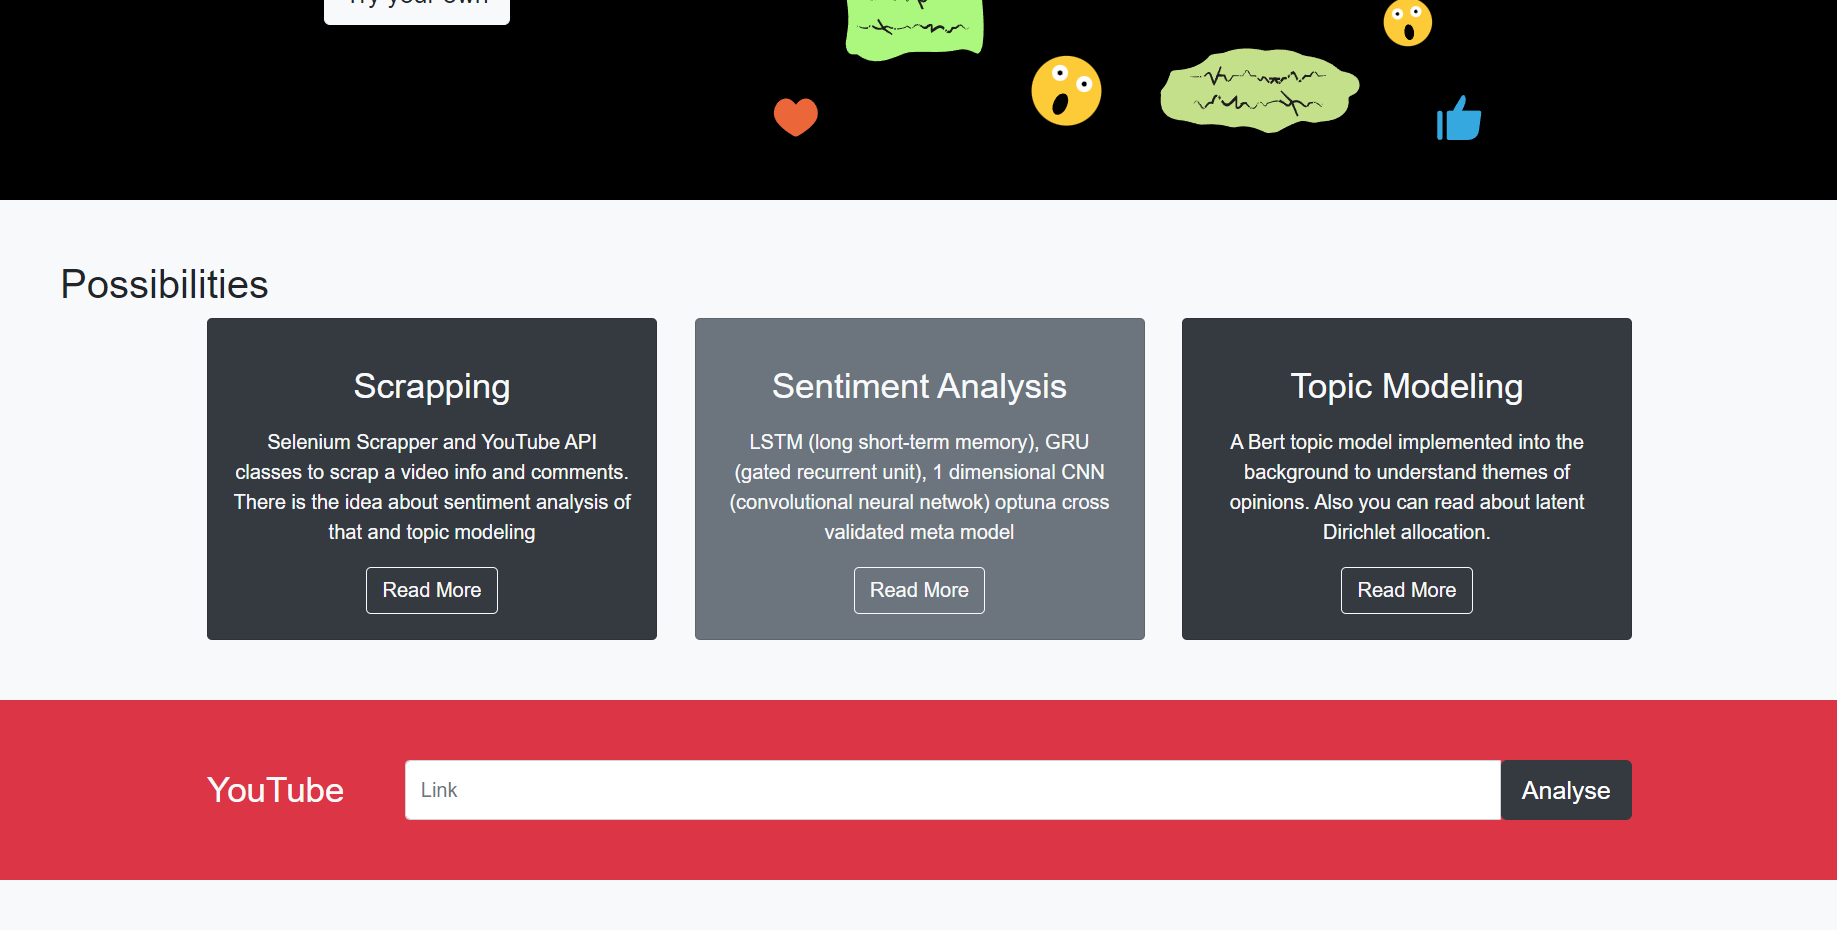
\includegraphics[scale=0.4]{web_mainpage-2.png}
    \caption{Главная страница сервиса}
    \label{fig:web2}
\end{figure}
\begin{figure}[H]
    \centering
    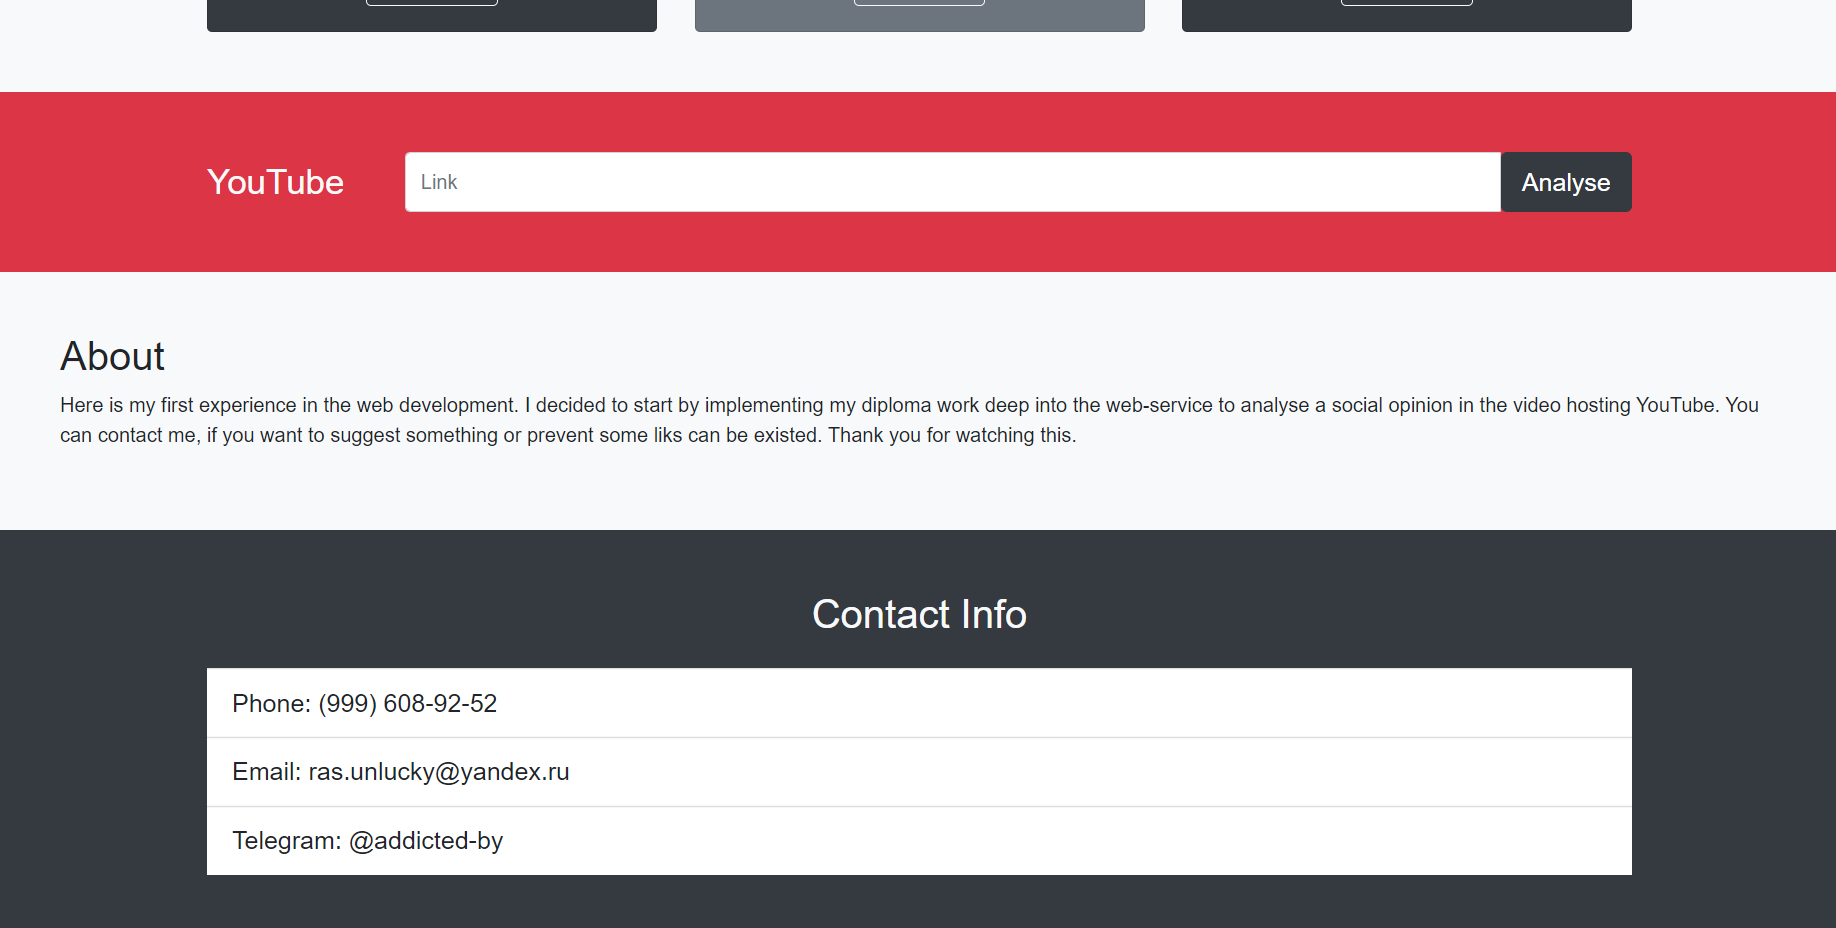
\includegraphics[scale=0.4]{web_mainpage_3.png}
    \caption{Главная страница. Поле ввода}
    \label{fig:web3}
\end{figure}
Как уже было сказано, реализованный сервис является кросплатформенным рис. \ref{fig:mobile}:
\begin{figure}[H]
    \centering
    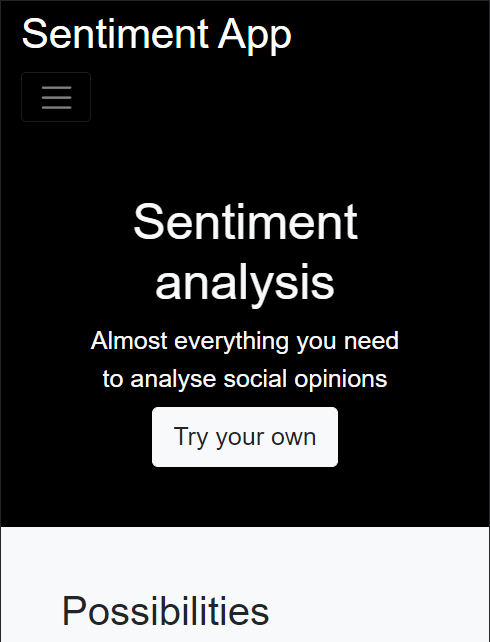
\includegraphics[scale=1.0]{mobile.png}
    \caption{Мобильная версия главной страницы}
    \label{fig:mobile}
\end{figure}
\begin{figure}[H]
    \centering
    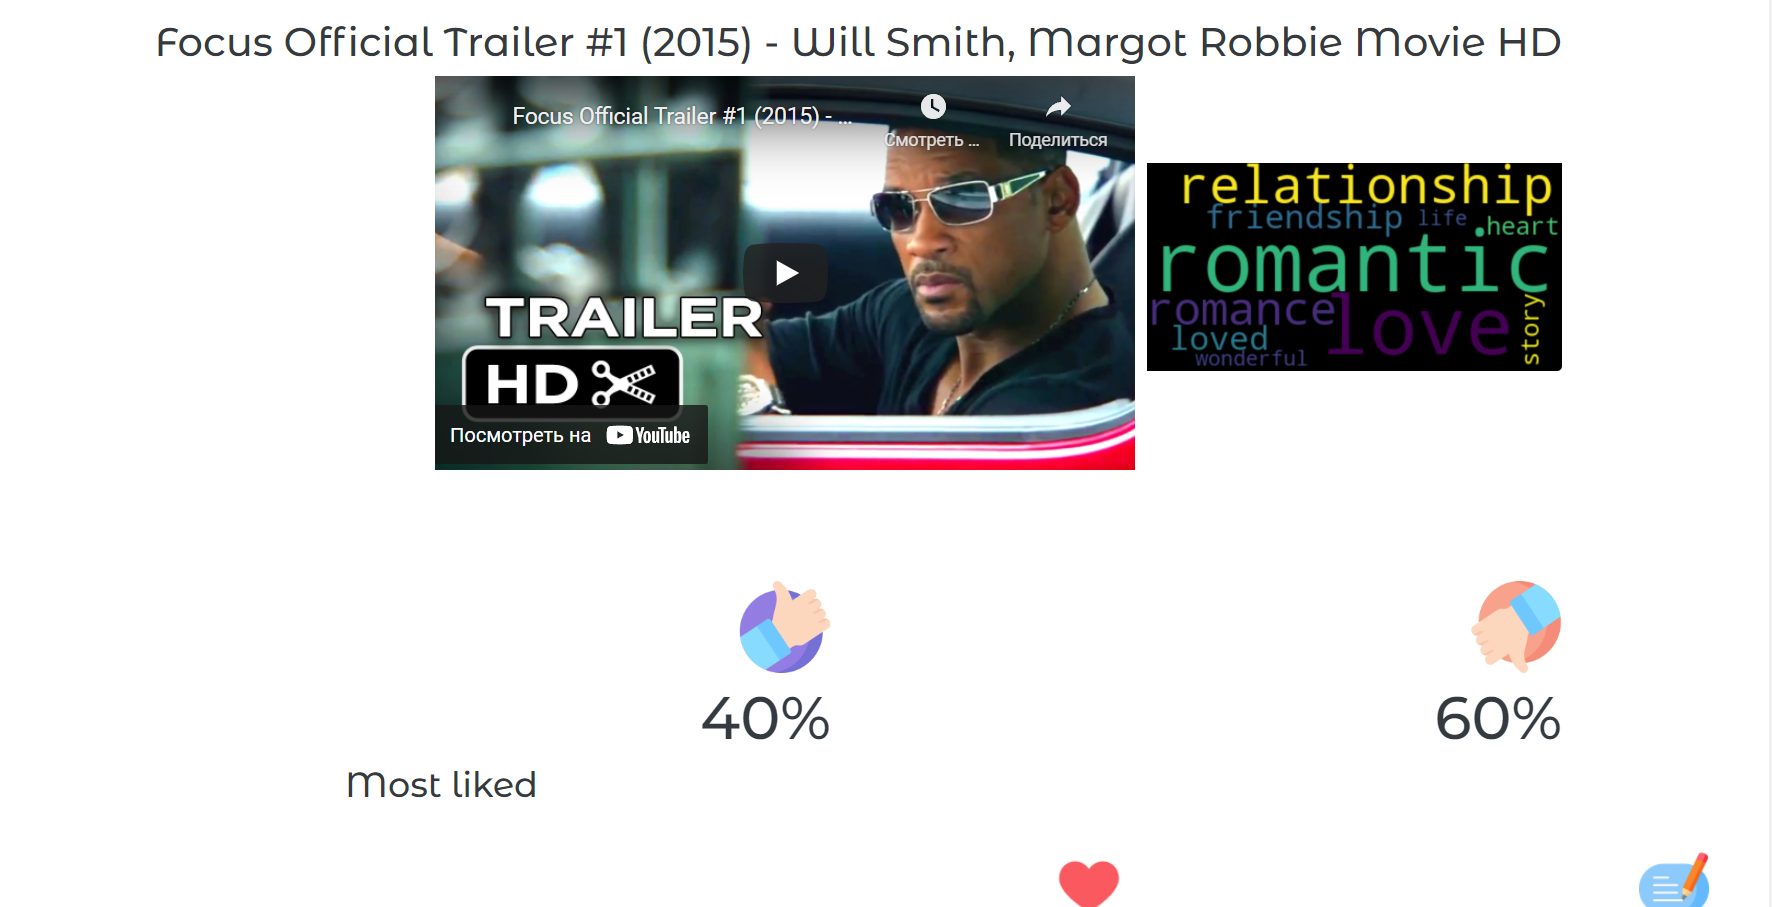
\includegraphics[scale=0.4]{web2.png}
    \caption{Страница анализа}
    \label{fig:web_analysis}
\end{figure}
Кроме того в процессе анализа можно посмотреть на самые интересующие публику (с наибольшим количеством лайков и ответов) комментарии (рис. \ref{fig:web_analysis2}).
\begin{figure}[H]
    \centering
    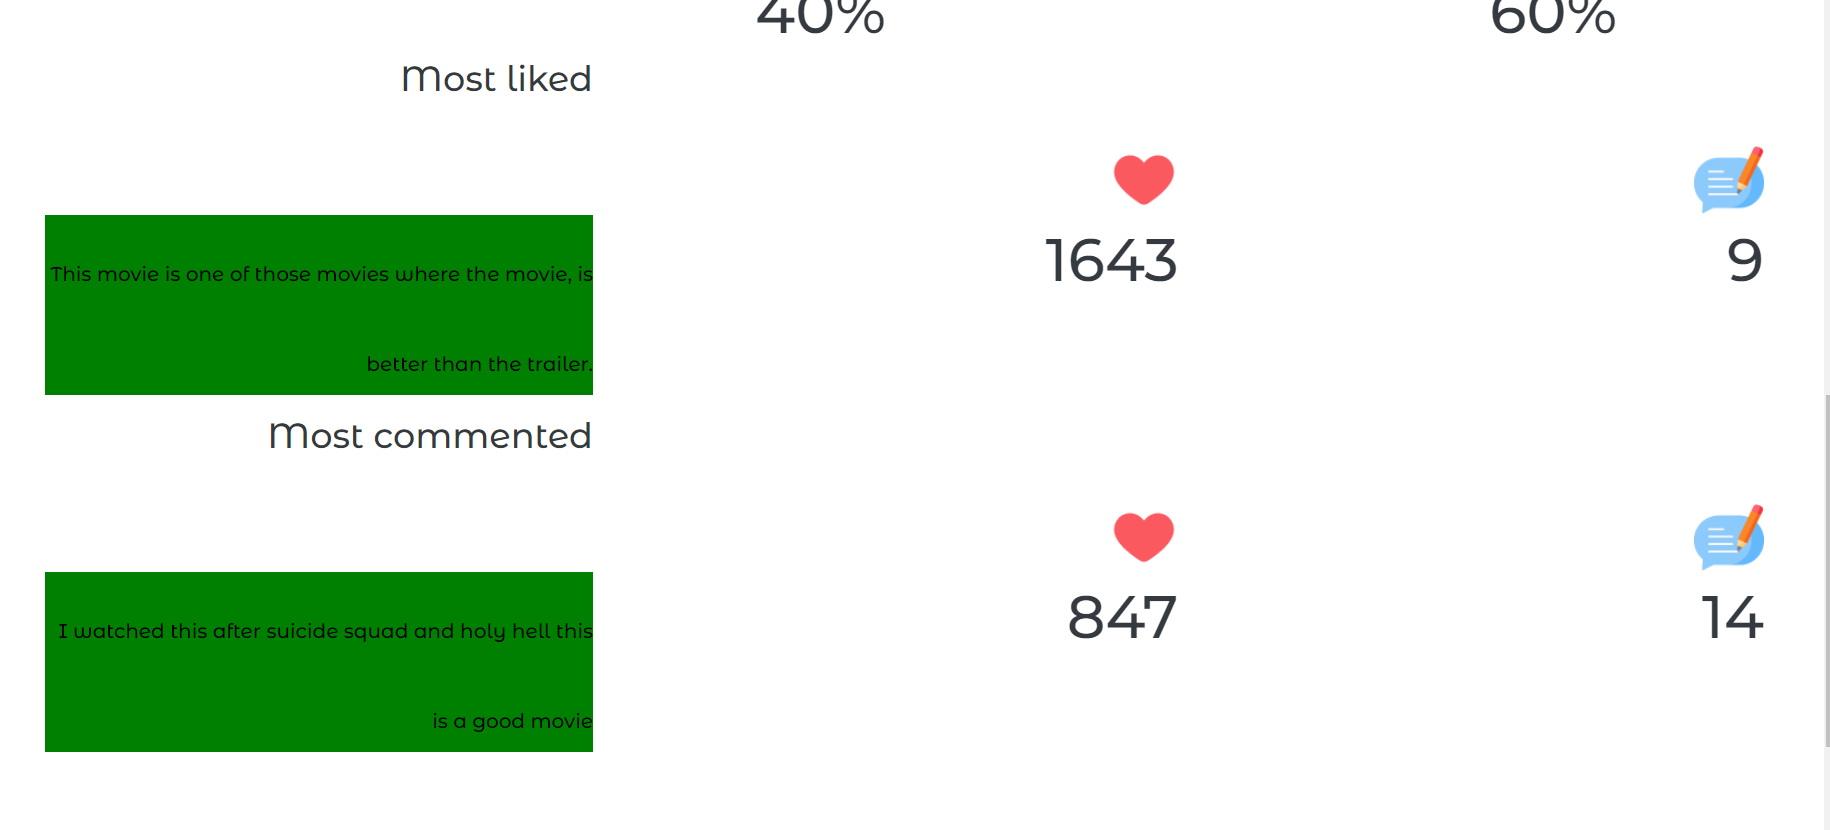
\includegraphics[scale=0.4]{web3.png}
    \caption{Страница анализа -- наиболее популярные комментарии}
    \label{fig:web_analysis2}
\end{figure}
